%%%%%%%%%%%%%%%%%%%%%%%
% AMS Talk
%%%%%%%%%%%%%%%%%%%%%%%
% Title Slide
{
\setbeamertemplate{background canvas}{bg=UniOrange;
\tikz[remember picture,overlay]
	\node[opacity=1] at (current page.center) {
	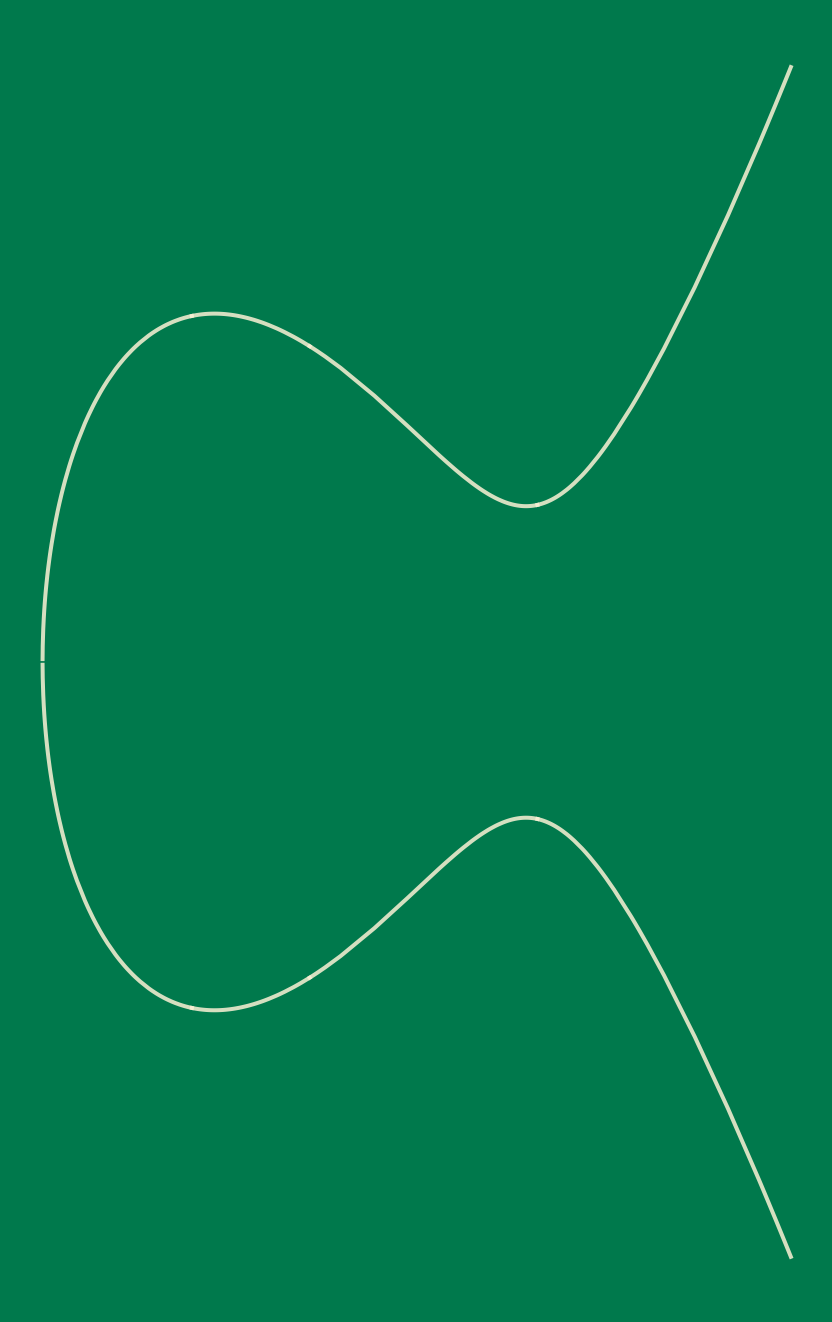
\includegraphics[width=1.05\paperwidth,
	height=\paperheight]{images/curve2.png}};} 
\begin{frame}[plain]
\phantom{.} \par\vspace{4.0cm}
\begin{center}
	{\Large\bfseries\color{UniGray} \textsc{Torsion Subgroups of Rational Elliptic Curves over Odd Degree Galois Fields}} 
\end{center} \vspace{1.5cm} 

\begin{center}
	{\bfseries\large\color{UniGray}\textit{Caleb McWhorter} \par
	\bfseries\textit{St. Thomas Aquinas College}} \par\vspace{0cm}
\end{center} 

\begin{center}
	{\bfseries\small\color{UniGray} October 1, 2022}
	\end{center} 
\end{frame}
}



%% Quote
%\begin{frame}[plain] 
%	\begin{minipage}{0.2\textwidth}
% 	\begin{figure}[h]
%	\centering
%	\fbox{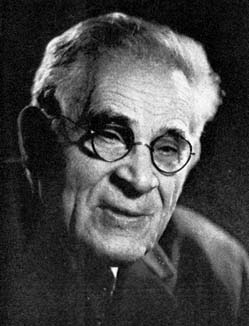
\includegraphics[width=1\textwidth]{images/mordell.jpg}} \par
%	{\small 1888--1972}
%	\end{figure}
%	\end{minipage}%
%	\begin{minipage}{0.8\textwidth}
%	\begin{center}
%	{\itshape ``Mathematicians have been familiar with very few questions for so long a period with so little accomplished in the way of general results, as that of finding the rational [points on elliptic curves].''} \\
%	 \phantom{x}\hfill-- L.J. Mordell, 1922
%	\end{center}
% 	\end{minipage}
%\end{frame}









% Mordell - Weil - Neron
\begin{frame}
	\begin{thm}[Mordell-Weil-N\'eron, 1952]
	Let $K$ be a field that is finitely generated over its prime field, and let $A/K$ be an abelian variety. Then the group of $K$-rational points on $A$, denoted $A(K)$, is a finitely generated abelian group. In particular,
		\[
		A(K) \cong \Z^{r_K} \oplus A(K)_\tors,
		\]
	where $r_K \geq 0$ is the rank and $A(K)_\tors$ is the torsion subgroup. 
	\end{thm}
	\begin{figure}[h]
	\centering
	\begin{subfigure}{0.3\textwidth}
	\captionsetup{labelformat=empty}
	\centering
	\fbox{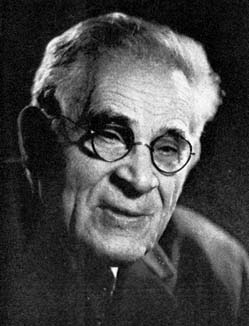
\includegraphics[width=0.8\textwidth]{images/mordell.jpg}}
	\caption{Louis J. Mordell}
	\end{subfigure}
	%
	\begin{subfigure}{0.3\textwidth}
	\captionsetup{labelformat=empty}
	\centering
	\fbox{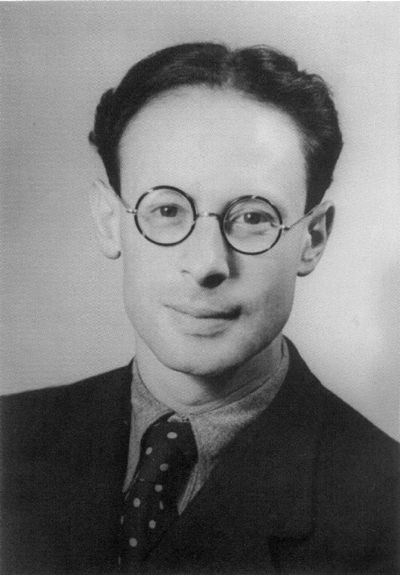
\includegraphics[width=0.74\textwidth]{images/weil.jpg}}
	\caption{Andr\'e Weil}
	\end{subfigure}
	%
	\begin{subfigure}{0.3\textwidth}
	\captionsetup{labelformat=empty}
	\centering
	\fbox{
\includegraphics[width=0.8\textwidth]{images/neron.png}}
	\caption{Andr\'e N\'eron}
	\end{subfigure}
	\end{figure}
\end{frame}



%% Torsion Subgroup
%\begin{frame}[plain]
%\ctext{Ranks of Elliptic Curves}
%\end{frame}
%
%
%
%
%
%% Rank Records
%\begin{frame}
%\begin{minipage}{0.62\textwidth}
%	\begin{tabular}{lll}  
%	{\itshape\large\bfseries Rank} & {\itshape\large\bfseries Year} & {\itshape\large\bfseries Due To} \\ \hline
%	3 & 1938 & Billing \\ \rowcolor{UniOrange}
%	\textcolor{white}{4} & \textcolor{white}{1945} &  \textcolor{white}{Wiman} \\ 
%	6 & 1974 & Penney/Pomerance \\ \rowcolor{UniOrange}
%	\textcolor{white}{7} & \textcolor{white}{1975} & \textcolor{white}{Penney/Pomerance} \\
%	8 & 1977 & Grunewald/Zimmert \\ \rowcolor{UniOrange}
%	\textcolor{white}{9} & \textcolor{white}{1977} & \textcolor{white}{Brumer/Kramer} \\
%	12 & 1982 & Mestre \\ \rowcolor{UniOrange}
%	\textcolor{white}{14} & \textcolor{white}{1986} & \textcolor{white}{Mestre} \\
%	15 & 1992 &  Mestre \\  \rowcolor{UniOrange}
%	\textcolor{white}{17} & \textcolor{white}{1992} & \textcolor{white}{Nagao} \\
%	19 & 1992 & Fermigier \\ \rowcolor{UniOrange}
%	\textcolor{white}{20} & \textcolor{white}{1993} & \textcolor{white}{Nagao} \\
%	21 & 1994 & Nagao/Kouya \\ \rowcolor{UniOrange}
%	\textcolor{white}{22} & \textcolor{white}{1997} & \textcolor{white}{Fermigier} \\
%	23 & 1998 & Martin/McMillen \\ \rowcolor{UniOrange}
%	\textcolor{white}{24} & \textcolor{white}{2000} & \textcolor{white}{Martin/McMillen} \\
%	28 & 2006 & Elkies 
%	\end{tabular}
%\end{minipage}%
%\begin{minipage}{0.20\textwidth}
%\centering
%	\begin{figure}
%	\begin{tikzpicture}[scale=0.30]%[scale=0.50, every node/.style={scale=0.1}]
%	\foreach \k in {0,...,15}
%		{
%		\draw (\k,0) -- (\k,15);
%		}
%	\foreach \k in {0,...,15}
%		{
%		\draw (0,\k) -- (15,\k);
%		}
%	\node at (0,-0.5) {\tiny 1900};
%	\node at (2,-0.5) {\tiny 1916};
%	\node at (4,-0.5) {\tiny 1932};
%	\node at (6,-0.5) {\tiny 1948};
%	\node at (8,-0.5) {\tiny 1964};
%	\node at (10,-0.5) {\tiny 1980};
%	\node at (12,-0.5) {\tiny 1996};
%	\node at (14,-0.5) {\tiny 2012};
%	
%	\node at (-0.5,0) {\tiny 0};
%	\node at (-0.5,1) {\tiny 2};
%	\node at (-0.5,2) {\tiny 4};
%	\node at (-0.5,3) {\tiny 6};
%	\node at (-0.5,4) {\tiny 8};
%	\node at (-0.5,5) {\tiny 10};
%	\node at (-0.5,6) {\tiny 12};
%	\node at (-0.5,7) {\tiny 14};
%	\node at (-0.5,8) {\tiny 16};
%	\node at (-0.5,9) {\tiny 18};
%	\node at (-0.5,10) {\tiny 20};
%	\node at (-0.5,11) {\tiny 22};
%	\node at (-0.5,12) {\tiny 24};
%	\node at (-0.5,13) {\tiny 26};
%	\node at (-0.5,14) {\tiny 28};
%	\node at (-0.5,15) {\tiny 30};
%	
%	\draw[very thick,red] plot[samples=500] coordinates {
%	(0,1)
%	(4.75,1.5)
%	(5.625,2)
%	(9.25,3)
%	(9.375,3.5)
%	(9.6667,4)
%	(9.7083,4.5)
%	(10.25,6)
%	(10.75,7)
%	(11.5313,7.5)
%	(11.5625,8.5)
%	(11.5938,9.5)
%	(11.625,10)
%	(11.75,10.5)
%	(12.125,11)
%	(12.25,11.5)
%	(12.5,12)
%	(13.25,14)
%	(14.875,14)
%	};
%	\end{tikzpicture}
%	\end{figure}
%\end{minipage}
%\end{frame}





% Torsion Subgroup
\begin{frame}[plain,fragile]
\ctext{Torsion Subgroups of Elliptic Curves} \small
\begin{tikzcd}[scale=0.5]
	& \left\{\begin{matrix} \text{Torsion Subgroups} \\ \text{of Elliptic Curves} \end{matrix} \right\} \arrow[<->]{dl} \arrow[<->]{dr} & \\
	\left\{\begin{matrix} \text{Galois} \\ \text{Representations} \end{matrix} \right\} \arrow[<->]{rr} & & \left\{\begin{matrix} \text{Modular} \\ \text{Curves} \end{matrix} \right\}
	\end{tikzcd}
\vfill
\end{frame}



%%%%%%%%%%%
% General Fields
%%%%%%%%%%%

%% Boundedness: Merel, Parent
%\begin{frame}[plain]
%\begin{thm}[Merel, 1996; Parent, 1999]
%Let $K$ be a number field of degree $d > 1$. Then
%	\begin{enumerate}[(i)]
%	\item (Merel) Let $E/K$ be an elliptic curve. If $E(K)$ contains a point of exact prime order $p$, then $\ell \leq d^{3d^2}$.
%	\item (Parent) If $P$ is a point of exact prime power order $\ell^n$, then
%		\begin{enumerate}[(a)]
%		\item $\ell^n \leq 65(3^d - 1)(2d)^6$, if $\ell \geq 5$
%		\item $\ell^n \leq 65(5^d - 1)(2d)^6$, if $\ell= 3$
%		\item $\ell^n \leq 129(3^d - 1)(3d)^6$, if $\ell= 2$
%		\end{enumerate}
%	In particular, $\ell^p \leq 129(5^d - 1)(3d)^6$ for all primes $\ell$. 
%	\item (Oesterl\'e) If $p \in S(d)$, then $p \leq (1 + 3^{d/2})^2$. 
%	\end{enumerate}
%\end{thm}
%	\begin{figure}[h]
%	\centering
%	\begin{subfigure}{0.3\textwidth}
%	\captionsetup{labelformat=empty}
%	\centering
%	\fbox{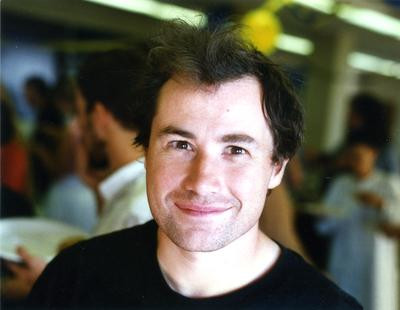
\includegraphics[width=0.92\textwidth]{images/merel.jpeg}}
%	\caption{Lo\"ic Merel}
%	\end{subfigure}
%	%
%	\begin{subfigure}{0.3\textwidth}
%	\captionsetup{labelformat=empty}
%	\centering
%	\fbox{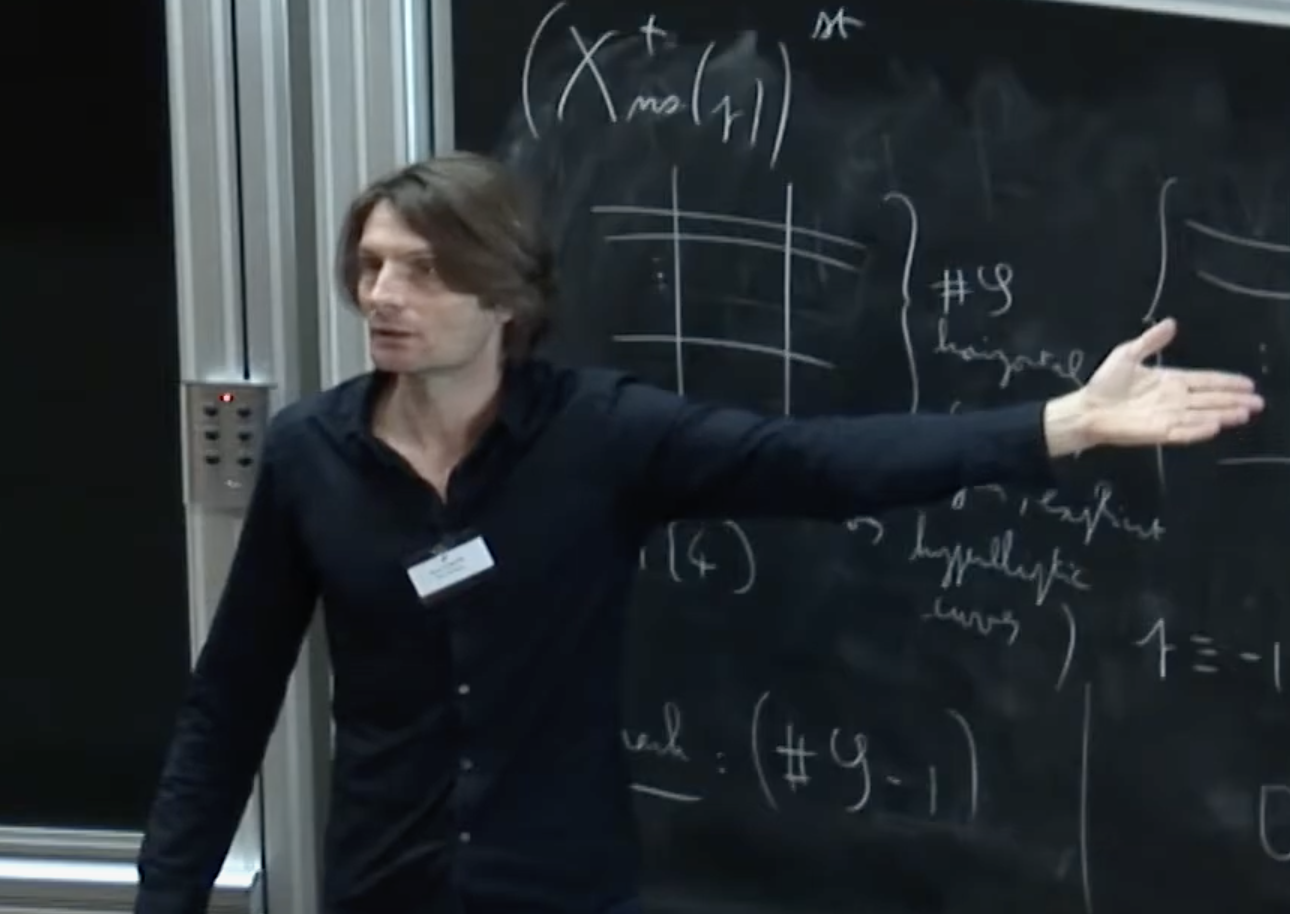
\includegraphics[width=\textwidth]{images/parent.png}}
%	\caption{Pierre Parent}
%	\end{subfigure} \hspace{0.05cm}
%	%
%	\begin{subfigure}{0.3\textwidth}
%	\captionsetup{labelformat=empty}
%	\centering
%	\fbox{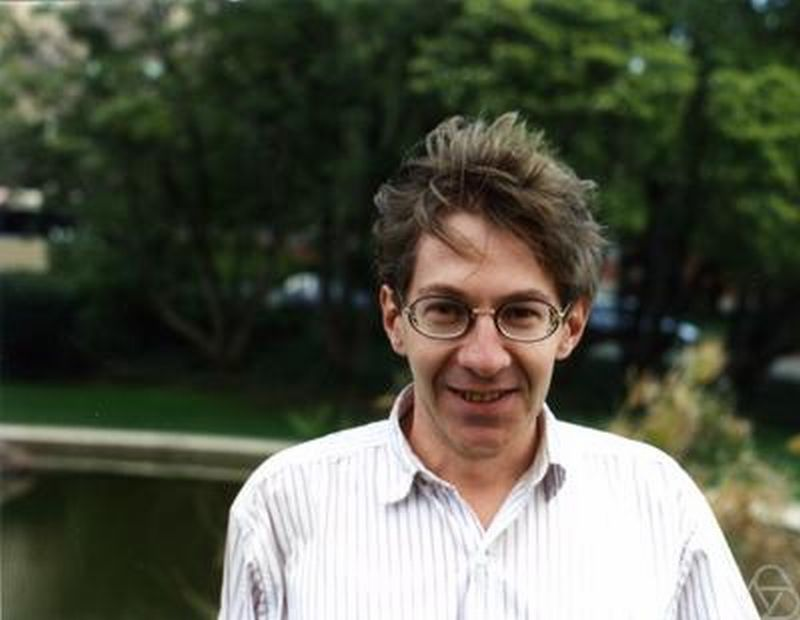
\includegraphics[width=0.92\textwidth]{images/oesterle.jpeg}}
%	\caption{Joseph Oesterl\'e}
%	\end{subfigure}
%	\end{figure}
%\end{frame}




% Q-Torsion (Mazur)
\begin{frame}[plain]
\begin{thm}[Levi-Ogg Conjecture; Mazur, 1977]
If $E/\Q$ is a rational elliptic curve, then the possible torsion subgroups $E(\Q)_\tors$ are precisely:
	\[
	\begin{cases}
	\Z/n\Z, & \text{with } n=1,2,\ldots,10,12 \text{ or} \\
	\Z/2\Z \oplus \Z/2n\Z, & \text{with } n=1,\ldots,4
	\end{cases}
	\]
Furthermore, each possibility occurs infinitely often.
\end{thm}
	\begin{figure}[h]
	\centering
	\begin{subfigure}{0.3\textwidth}
	\captionsetup{labelformat=empty}
	\centering
	\fbox{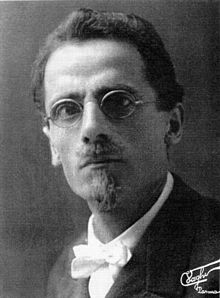
\includegraphics[width=0.72\textwidth]{images/levi.jpg}}
	\caption{Beppo Levi}
	\end{subfigure}
	%
	\begin{subfigure}{0.3\textwidth}
	\captionsetup{labelformat=empty}
	\centering
	\fbox{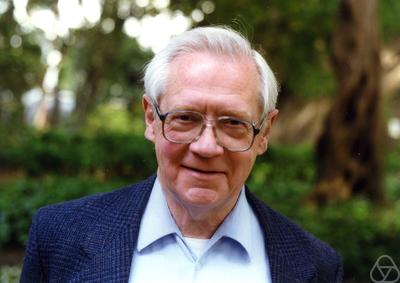
\includegraphics[width=\textwidth]{images/ogg.jpg}}
	\caption{Andrew Ogg}
	\end{subfigure} \hspace{0.05cm}
	%
	\begin{subfigure}{0.3\textwidth}
	\captionsetup{labelformat=empty}
	\centering
	\fbox{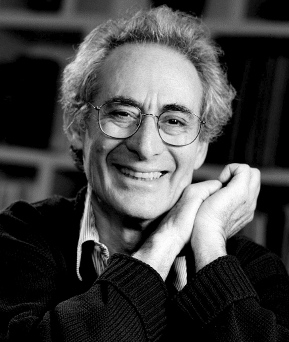
\includegraphics[width=0.83\textwidth]{images/mazur.jpg}}
	\caption{Barry Mazur}
	\end{subfigure}
	\end{figure}
\end{frame}




% Degree d Number Fields
\begin{frame}[plain]
\ctext{What about number fields of degree $d$?}
\end{frame}


% Joke
\begin{frame}[plain]
\ctext{With massive loss of generality, let $d= 2$.}
\end{frame}


% Quadratic Number Field
\begin{frame}[plain]
\begin{thm}[Kenku, Momose, 1988; Kamienny, 1992]
 Let $K/\Q$ be a quadratic number field and $E/K$ be an elliptic curve. Then the possible torsion subgroups $E(K)_\tors$ are precisely:
 	\[
	\begin{cases}
	\Z/n\Z, & \text{with } n=1,2,\ldots,16,18 \text{ or} \\
	\Z/2\Z \oplus \Z/2n\Z, & \text{with } n=1,\ldots,6 \text{ or} \\
	\Z/3\Z \oplus \Z/3n\Z, & \text{with } n=1,2 \text{ or} \\
	\Z/4\Z \oplus \Z/4\Z
	\end{cases}
	\]
Moreover, each possibility occurs infinitely often. 
\end{thm}
	\begin{figure}[h]
	\centering
	\begin{subfigure}{0.3\textwidth}
	\captionsetup{labelformat=empty}
	\centering
	\fbox{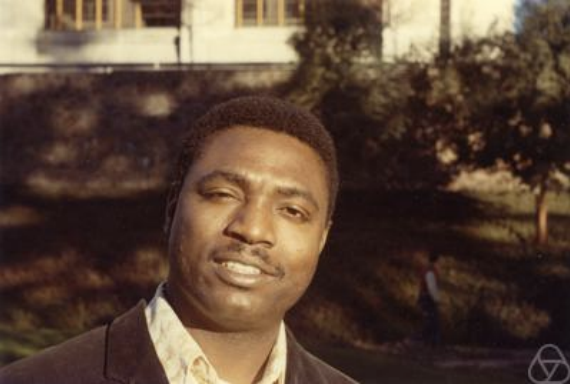
\includegraphics[width=0.9\textwidth]{images/kenku.png}}
	\caption{Monsur Kenku}
	\end{subfigure} \;\;\;
	%
	\begin{subfigure}{0.3\textwidth}
	\captionsetup{labelformat=empty}
	\centering
	\fbox{
\includegraphics[width=0.85\textwidth]{images/momose.png}}
	\caption{Fumiyuki Momose}
	\end{subfigure}
	%
	\begin{subfigure}{0.3\textwidth}
	\captionsetup{labelformat=empty}
	\centering
	\fbox{
\includegraphics[width=0.63\textwidth]{images/kamienny.png}}
	\caption{Sheldon Kamienny}
	\end{subfigure}
	\end{figure}
\end{frame}





% Cubic Number Field
\begin{frame}[plain,c]
\footnotesize
\begin{thm}[Jeon,Kim,Schweizer, 2004; Etropolski,Morrow,Zureick Brown; Derickx, 2016; Derickx,Etropolski,van Hoeij,Morrow,Zureick-Brown, 2020]
Let $K/\Q$ be a cubic number field and $E/K$ be an elliptic curve. Then the possible torsion subgroups $E(K)_\tors$ are precisely:
	\[
	\begin{cases}
	\Z/n\Z, & \text{with } n=1,2,\ldots,16,18,20,21 \text{ or} \\
	\Z/2n\Z, & \text{with }n=1,\ldots,7
	\end{cases}
	\] 
Each of these possibilities occurs infinitely many times except for $\Z/21\Z$ which occurs only for the elliptic curve \texttt{162b1} over $\Q(\zeta_9)^+$.
\end{thm}
	\begin{figure}[h]
	\centering
	\begin{subfigure}{0.10\textwidth}
	\captionsetup{labelformat=empty}
	\centering
	\fbox{
\includegraphics[width=1.2\textwidth]{images/jeon.png}}
	\caption{\hspace{0.2cm}\scriptsize{Jeon}}
	\end{subfigure} \quad\quad
	%
	\begin{subfigure}{0.10\textwidth}
	\captionsetup{labelformat=empty}
	\centering
	\fbox{
\includegraphics[width=1.2\textwidth]{images/kim.jpg}}
	\caption{\hspace{0.3cm}\scriptsize{Kim}}
	\end{subfigure} \quad\quad
	%
	\begin{subfigure}{0.10\textwidth}
	\captionsetup{labelformat=empty}
	\centering
	\fbox{
\includegraphics[width=1.2\textwidth]{images/schweizer.jpeg}}
	\caption{\hspace{0.1cm}\scriptsize{Schweizer}}
	\end{subfigure} \\
	%
	\hfill
	\begin{subfigure}{0.12\textwidth}
	\captionsetup{labelformat=empty}
	\centering
	\fbox{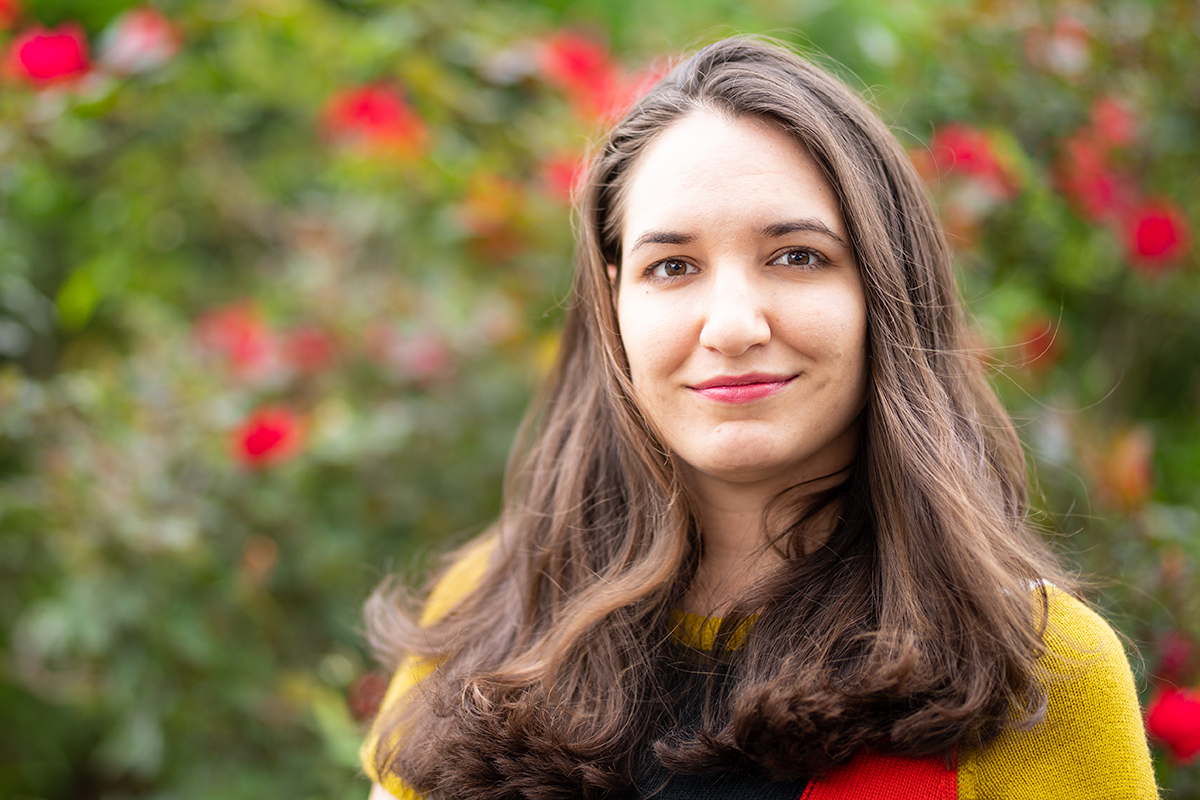
\includegraphics[width=1.7\textwidth]{images/etropolski.jpg}}
	\caption{\;\;\;\;\scriptsize{Etropolski}}
	\end{subfigure} \hspace{1.5cm}
	%
	\begin{subfigure}{0.10\textwidth}
	\captionsetup{labelformat=empty}
	\centering
	\fbox{
\includegraphics[width=1.45\textwidth]{images/morrow.png}}
	\caption{\;\;\;\scriptsize{Morrow}}
	\end{subfigure} \hspace{0.6cm}
	%
	\begin{subfigure}{0.192\textwidth}
	\captionsetup{labelformat=empty}
	\centering
	\fbox{
\includegraphics[width=0.55\textwidth]{images/zbrown3.jpeg}}
	\caption{\scriptsize Zureick-Brown}
	\end{subfigure} \hspace{0cm}
	%
	\begin{subfigure}{0.09\textwidth}
	\captionsetup{labelformat=empty}
	\centering
	\fbox{
\includegraphics[width=1.2\textwidth]{images/derickx.jpg}}
	\caption{\;\;\scriptsize{Derickx}}
	\end{subfigure} \hfill \phantom{.}
	\begin{subfigure}{0.115\textwidth}
	\captionsetup{labelformat=empty}
	\centering
	\fbox{
\includegraphics[width=1.2\textwidth]{images/hoeij.jpeg}}
	\caption{\;\;\tiny{van Hoeij}}
	\end{subfigure} \hfill \phantom{.}
	\end{figure}
\end{frame}





% Quartic Number Field
\begin{frame}[plain]
\begin{thm}[Jeon, Kim, Park, 2006]
Let $K/\Q$ be a quartic number field and $E/K$ be an elliptic curve. Then the possible torsion subgroups $E(K)_\tors$ appearing infinitely often are precisely:
	\[
	\begin{cases}
	\Z/n\Z, & \text{with } n=1,2,\ldots,18,20,21,22 \text{ or} \\
	\Z/2\Z \oplus \Z/2n\Z, & \text{with } n=1,\ldots,9 \text{ or} \\
	\Z/3\Z \oplus \Z/3n\Z, & \text{with } n=1,2,3 \text{ or} \\
	\Z/4\Z \oplus \Z/4n\Z, & \text{with } n=1,2 \text{ or} \\
	\Z/5\Z \oplus \Z/5\Z & \text{ or} \\
	\Z/6\Z \oplus \Z/6\Z
	\end{cases}
	\]
\end{thm}
	\begin{figure}[h]
	\centering
	\begin{subfigure}{0.3\textwidth}
	\captionsetup{labelformat=empty}
	\centering
	\fbox{
\includegraphics[width=0.60\textwidth]{images/jeon.png}}
	\caption{\hspace{0.1cm}Daeyeol Jeon}
	\end{subfigure}
	%
	\begin{subfigure}{0.3\textwidth}
	\captionsetup{labelformat=empty}
	\centering
	\fbox{
\includegraphics[width=0.63\textwidth]{images/kim.jpg}}
	\caption{Chang Kim}
	\end{subfigure}
	%
	\begin{subfigure}{0.3\textwidth}
	\captionsetup{labelformat=empty}
	\centering
	\fbox{
\includegraphics[width=0.45\textwidth]{images/park.png}}
	\caption{\hspace{0cm}Eui-Sung Park}
	\end{subfigure}
	\end{figure}
\end{frame}



% Quintic Number Field
\begin{frame}[plain]
\begin{thm}[Derickx, Sutherland, 2016]
Let $K/\Q$ be a quintic number field and $E/K$ be an elliptic curve. Then the possible torsion subgroups $E(K)_\tors$ appearing infinitely often are precisely:
	\[
	\begin{cases}
	\Z/n\Z, & \text{with } n=1,\ldots,22,24,25 \text{ or} \\
	\Z/2\Z \oplus \Z/2n\Z, & \text{with } n=1,\ldots,8
	\end{cases}
	\]
\end{thm}
	\begin{figure}[h]
	\centering
	\begin{subfigure}{0.3\textwidth}
	\captionsetup{labelformat=empty}
	\centering
	\fbox{
\includegraphics[width=0.72\textwidth]{images/derickx.jpg}}
	\caption{\hspace{0.1cm}Maarten Derickx}
	\end{subfigure}
	%
	\begin{subfigure}{0.3\textwidth}
	\captionsetup{labelformat=empty}
	\centering
	\fbox{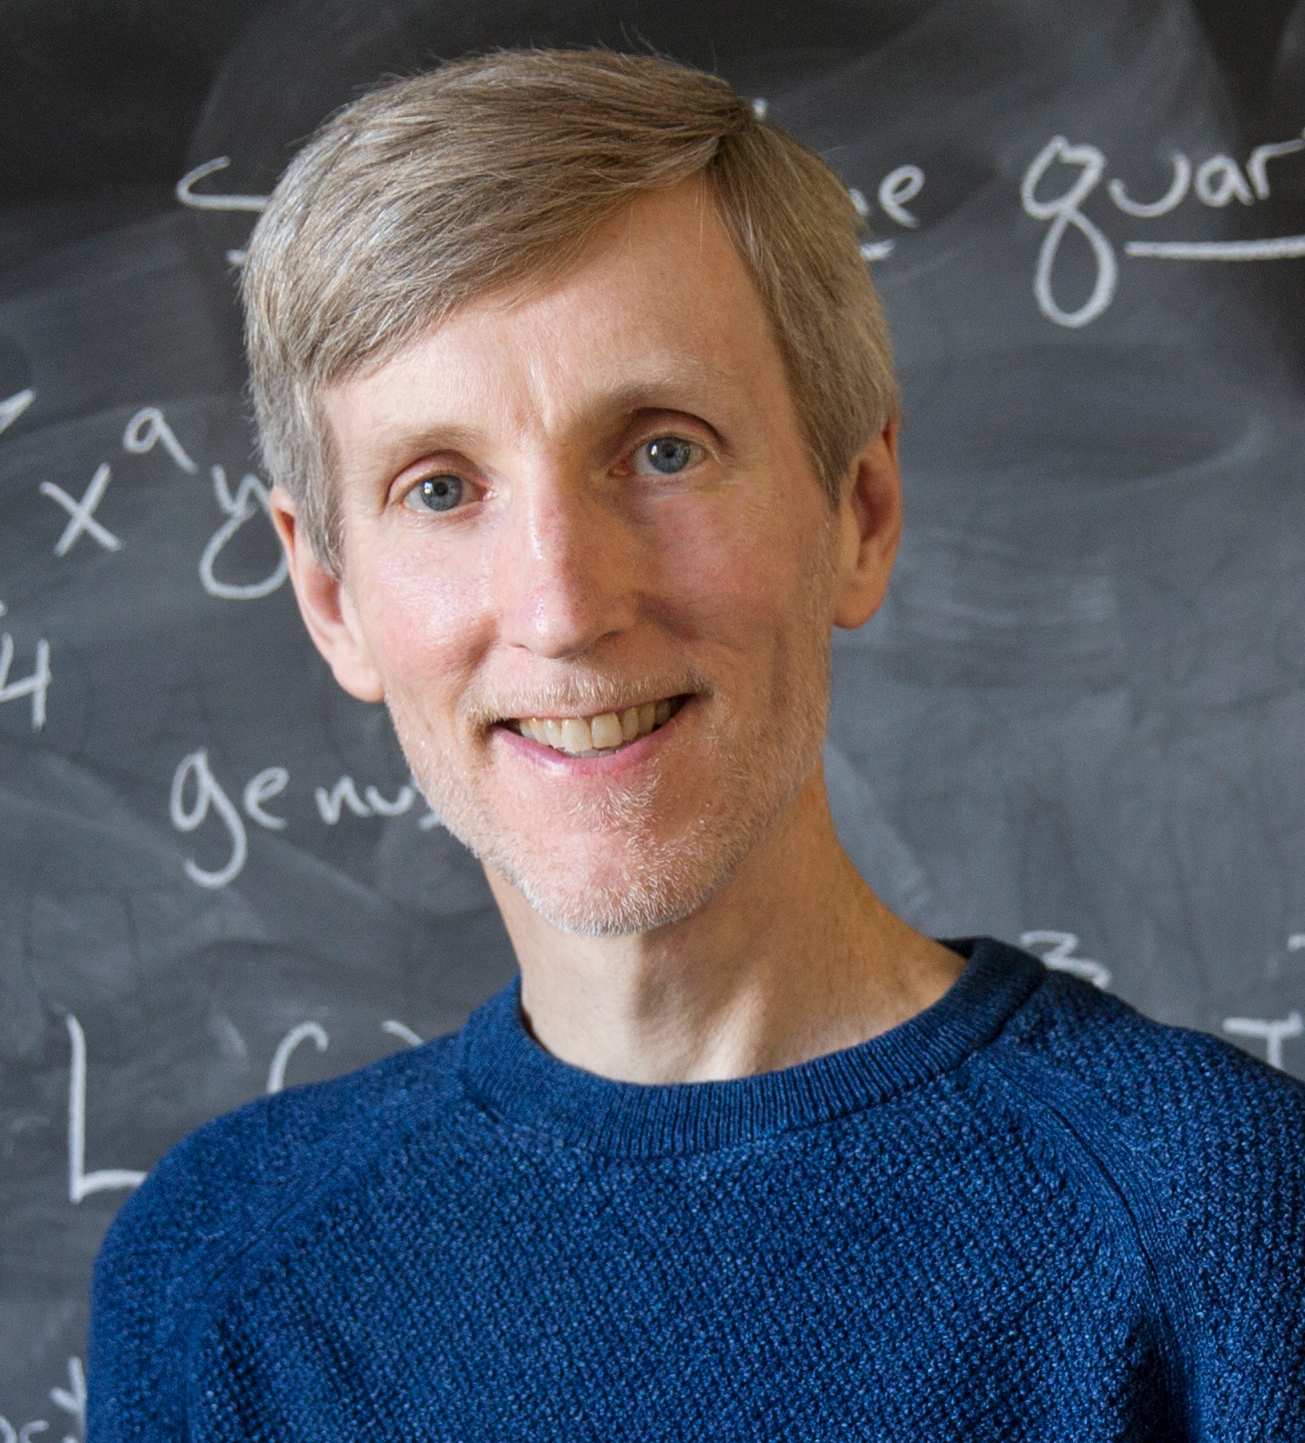
\includegraphics[width=0.82\textwidth]{images/sutherland.jpg}}
	\caption{Drew Sutherland}
	\end{subfigure}
	\end{figure}
\end{frame}



% Sextic Number Field
\begin{frame}[plain]
\begin{thm}[Derickx, Sutherland, 2016]
Let $K/\Q$ be a sextic number field and $E/K$ be an elliptic curve. Then the possible torsion subgroups $E(K)_\tors$ appearing infinitely often are precisely:
	\[
	\begin{cases}
	\Z/n\Z, &  \text{with } n=1,\ldots,30; n \neq 23,25,29 \text{ or} \\
	\Z/2\Z \oplus \Z/2n\Z, & \text{with } n=1,\ldots,10 \text{ or} \\
	\Z/3\Z \oplus \Z/3n\Z, & \text{with } n=1,\ldots,4 \text{ or} \\
	\Z/4\Z \oplus \Z/4n\Z, & \text{with } n=1,2 \text{ or} \\
	\Z/6\Z \oplus \Z/6\Z 
	\end{cases}
	\]
\end{thm}
	\begin{figure}[h]
	\centering
	\begin{subfigure}{0.28\textwidth}
	\captionsetup{labelformat=empty}
	\centering
	\fbox{
\includegraphics[width=0.72\textwidth]{images/derickx.jpg}}
	\caption{\hspace{0.1cm}Maarten Derickx}
	\end{subfigure}
	%
	\begin{subfigure}{0.28\textwidth}
	\captionsetup{labelformat=empty}
	\centering
	\fbox{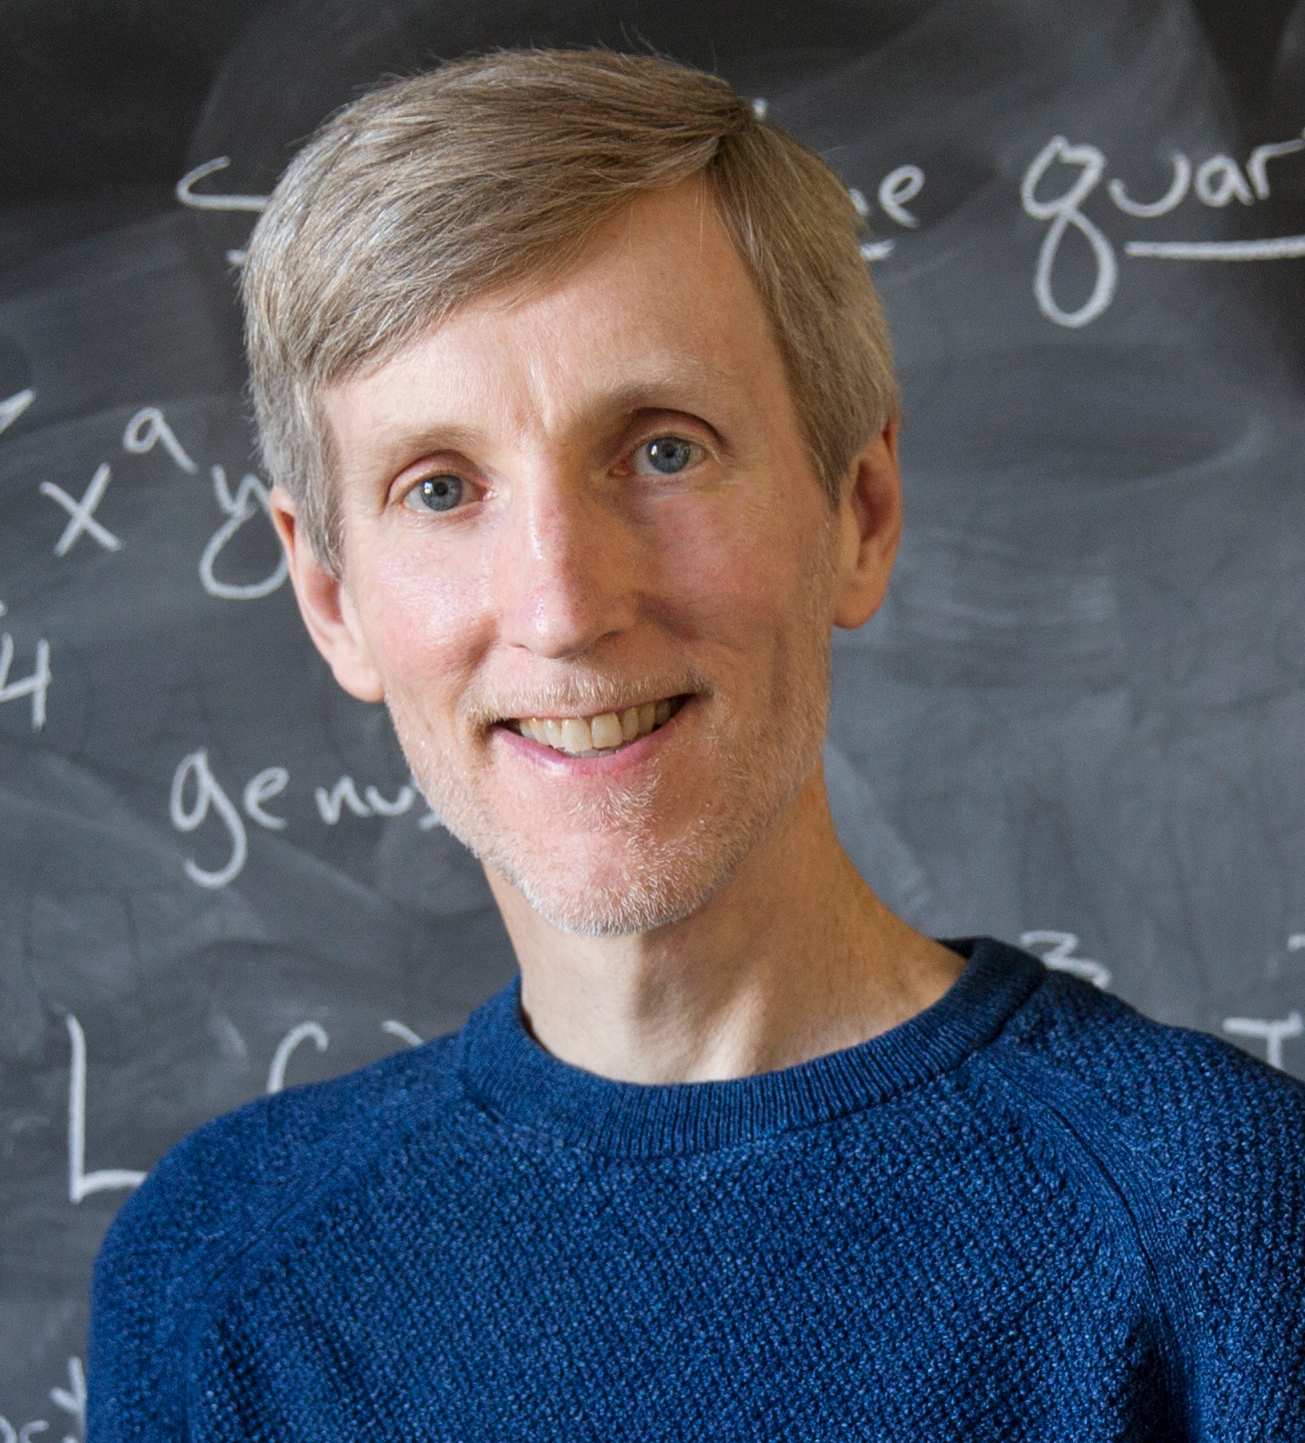
\includegraphics[width=0.82\textwidth]{images/sutherland.jpg}}
	\caption{Drew Sutherland}
	\end{subfigure}
	\end{figure}
\end{frame}







%%%%%%%%%%%
% CM Curves
%%%%%%%%%%%

\begin{frame}[plain,c]
\ctext{What about CM Elliptic Curves?}
\end{frame}

% CM Clark, Corn, Rice, Stankewicz
\begin{frame}[plain,c]
	\begin{thm}[Clark, Corn, Rice, Stankewicz; 2013]
	Let $K$ be a number field of degree $d=1,2,\ldots,13$ and $E/K$ be an elliptic curve with CM. Then all possible torsion subgroups are given, and an algorithm to compute the list.
	\end{thm} 
	\begin{figure}[h]
	\centering
	\begin{subfigure}{0.23\textwidth}
	\captionsetup{labelformat=empty}
	\centering
	\fbox{
\includegraphics[width=0.75\textwidth]{images/clark.jpg}}
	\caption{Pete Clark}
	\end{subfigure}
	%
	\begin{subfigure}{0.23\textwidth}
	\captionsetup{labelformat=empty}
	\centering
	\fbox{
\includegraphics[width=0.83\textwidth]{images/corn.jpg}}
	\caption{Patrick Corn}
	\end{subfigure}
	%
	\begin{subfigure}{0.23\textwidth}
	\captionsetup{labelformat=empty}
	\centering
	\fbox{
\includegraphics[width=1.0\textwidth]{images/rice.png}}
	\caption{Alex Rice}
	\end{subfigure}
	%
	\begin{subfigure}{0.25\textwidth}
	\captionsetup{labelformat=empty}
	\centering
	\fbox{
\includegraphics[width=0.65\textwidth]{images/stankewicz.png}}
	\caption{James Stankewicz}
	\end{subfigure}
	\end{figure}
\end{frame}




% CM Bourdon Clark Stankewicz
\begin{frame}[plain]
\footnotesize
\begin{thm}[Bourdon, Clark, Stankewicz, 2015]
Let $F$ be a number field of odd degree, let $E/F$ be a $K$-CM elliptic curve, and let $T= E(F)_\tors$. Then
	\begin{enumerate}[(a)]
	\item One of the following occurs:
		\begin{enumerate}[(i)] \footnotesize
		\item $T$ is isomorphic to the trivial group $\O$, $\Z/2\Z$, $\Z/4\Z$, or $\Z/2\Z \times \Z/2\Z$;
		\item $T \cong \Z/\ell^n\Z$ for a prime $\ell \equiv 3 \mod 8$ and $n \in \Z^+$ and $K= \Q(\sqrt{-\ell})$;
		\item $T \cong \Z/2\ell^n\Z$ for a prime $\ell \equiv 3 \mod 4$ and $n \in \Z^+$ and $K= \Q(\sqrt{-\ell})$. 
		\end{enumerate}
	\item If $E(F)_\tors \cong \Z/2\Z \oplus \Z/2\Z$, then $\End E$ has discriminant $\Delta= -4$.
	\item If $E(F)_\tors \cong \Z/4\Z$, then $\End E$ has discriminant $\Delta \in \{ -4, -16 \}$.
	\item Each of the groups listed in part (a) arises up to isomorphism as the torsion subgroup $E(F)$ of a CM elliptic curve $E$ defined over an odd degree number field $F$. 
	\end{enumerate}
\end{thm}
	\begin{figure}[h]
	\centering
	\begin{subfigure}{0.30\textwidth}
	\captionsetup{labelformat=empty}
	\centering
	\fbox{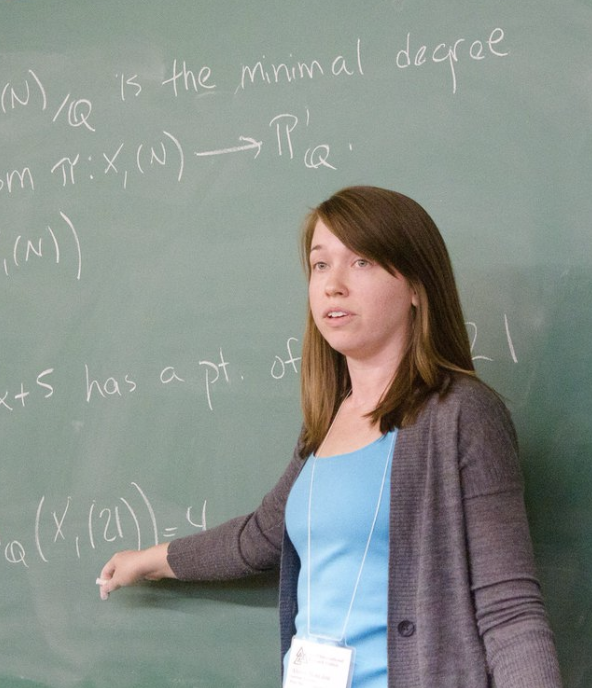
\includegraphics[width=0.65\textwidth]{images/bourdon.png}}
	\caption{\scriptsize Abbey Bourdon}
	\end{subfigure}
	%
	\begin{subfigure}{0.30\textwidth}
	\captionsetup{labelformat=empty}
	\centering
	\fbox{
\includegraphics[width=0.56\textwidth]{images/clark.jpg}}
	\caption{\scriptsize Pete Clark}
	\end{subfigure}
	%
	\begin{subfigure}{0.30\textwidth}
	\captionsetup{labelformat=empty}
	\centering
	\fbox{
\includegraphics[width=0.53\textwidth]{images/stankewicz.png}}
	\caption{\scriptsize James Stankewicz}
	\end{subfigure}
	\end{figure}
\end{frame}





% CM Bourdon Pollack
\begin{frame}[plain]
	\begin{thm}[Bourdon, Pollack; 2018]
	Let $K$ be an odd degree number field and $E/K$ be an elliptic curve with CM. Then the torsion subgroups $E(K)_\tors$ are computable. 
	\end{thm} 
	\begin{figure}[h]
	\centering
	\begin{subfigure}{0.3\textwidth}
	\captionsetup{labelformat=empty}
	\centering
	\fbox{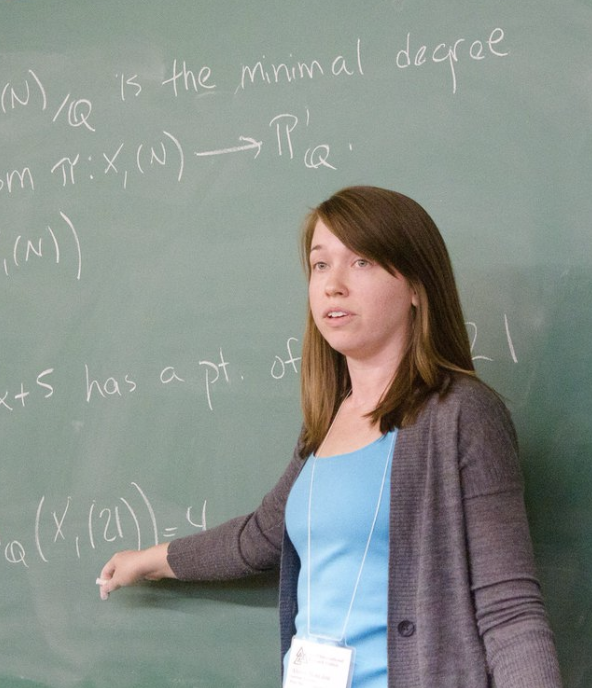
\includegraphics[width=0.85\textwidth]{images/bourdon.png}}
	\caption{Abbey Bourdon}
	\end{subfigure}
	%
	\begin{subfigure}{0.3\textwidth}
	\captionsetup{labelformat=empty}
	\centering
	\fbox{
\includegraphics[width=0.82\textwidth]{images/pollack.jpg}}
	\caption{Paul Pollack}
	\end{subfigure}
	\end{figure}
\end{frame}



% CM Bourdon Pollack
\begin{frame}[plain]
\tiny
\begin{thm}[Bourdon, Chaos; 2022]
Let $F$ be a number field of degree $2p$ for $p > 5$ prime, and let $E/F$ be an elliptic curve with CM by the order of discriminant $\Delta$. Then $E(F)_\tors$ is new if and only if one of the following occurs:
	\begin{enumerate}[(i)]
	\item $\Delta= -115$, $p= 11$, and $E(F)_\tors \cong \Z/23\Z$, or 
	\item $\Delta= -235$, $p= 23$, and $E(F)_\tors \cong \Z/47\Z$, or
	\item $\Delta= \in \{ -11, -19, -27, -43, -67, -163 \}$, $p$ is a Germain prime with $\left( \dfrac{\Delta}{2p + 1} \right)= 1$, and $E(F)_\tors \cong \Z/(2p + 1)\Z$, or
	\item $\Delta \in \{ -8, -12, -16, -28 \}$, $p$ is a Germain prime with $\left( \dfrac{\Delta}{2p + 1} \right)= 1$, and $E(F)_\tors \cong \Z/2(2p + 1)\Z$, or 
	\item $\Delta= -7$, $p$ is a Germain prime with $\left( \dfrac{\Delta}{2p + 1} \right)= 1$, and $E(F)_\tors \cong \Z/2\Z \oplus \Z 2(2p + 1)\Z$, or
	\item $\Delta= -3$, $p= 7$, and $E(F)_\tors \cong \Z/49\Z$, or 
	\item $\Delta= -3$, $6p + 1$ is prime, and $E(F)_\tors \cong \Z/(6p + 1)\Z$, or
	\item $\Delta= -4$, $4p + 1$ is prime, and $E(F)_\tors \cong \Z/2(4p + 1)\Z$. 
	\end{enumerate}
In particular, any new torsion subgroup arises on one of only finitely many CM elliptic curves, and all but $\Delta= -115$ and $-235$ correspond to imaginary quadratic orders of class number 1. 
\end{thm} 

	\begin{figure}[h]
	\centering
	\begin{subfigure}{0.3\textwidth}
	\captionsetup{labelformat=empty}
	\centering
	\fbox{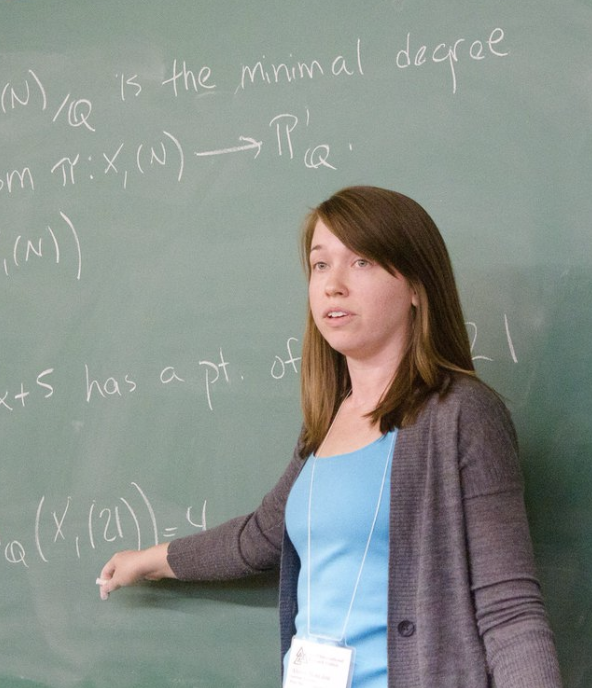
\includegraphics[width=0.59\textwidth]{images/bourdon.png}}
	\caption{\scriptsize Abbey Bourdon}
	\end{subfigure}
	%
	\begin{subfigure}{0.3\textwidth}
	\captionsetup{labelformat=empty}
	\centering
	\fbox{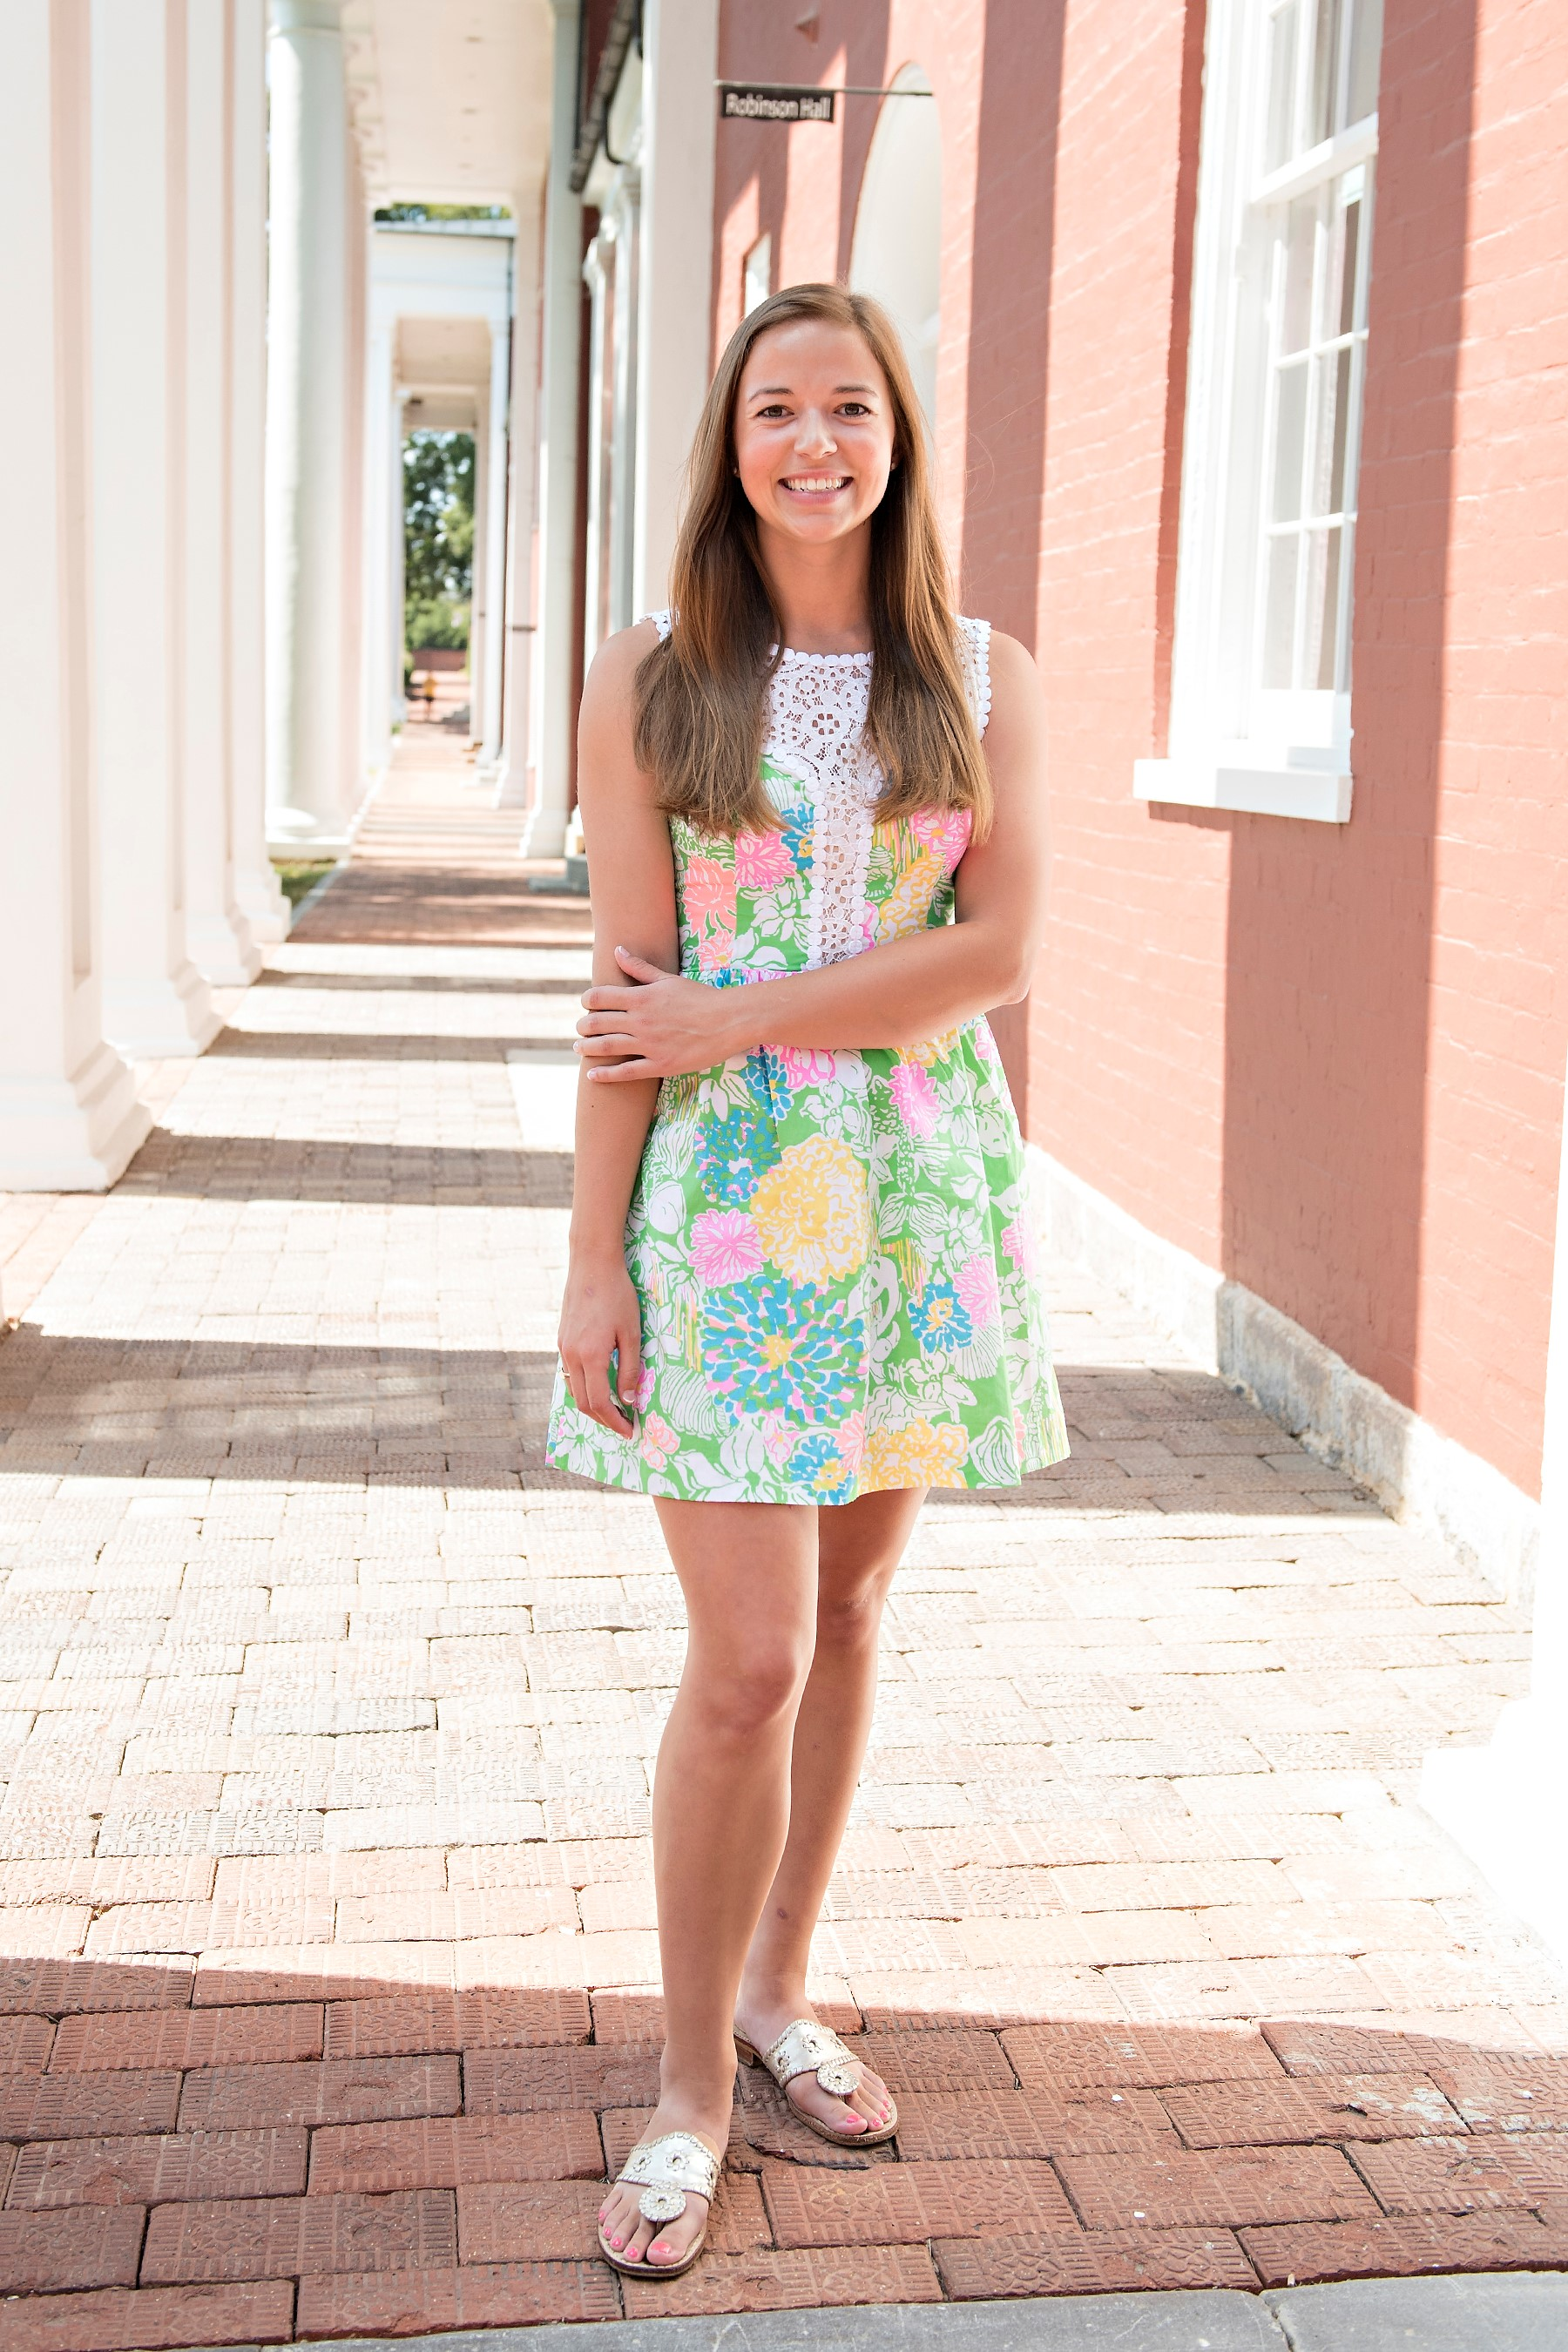
\includegraphics[width=0.465\textwidth]{images/chaos.jpeg}}
	\caption{\scriptsize Holly Paige Chaos}
	\end{subfigure}
	\end{figure}
\end{frame}


% Rational Elliptic Curves
\begin{frame}[plain]
\ctext{What about elliptic curves $E/\Q$?}
\end{frame}



%%%%%%%%%%%
% Rational Elliptic 
%%%%%%%%%%%

% Quadratic Rational EC
\begin{frame}[plain]
\footnotesize
\begin{thm}[Najman, 2015]
Let $E/\Q$ be a rational elliptic curve, and let $K/\Q$ be a quadratic number field. Then the possible torsion subgroups $E(K)_\tors$ are precisely:
	\[
	\begin{cases}
	\Z/n\Z, & \text{with } n= 1, 2, \ldots, 10, 12, 15, 16 \text{ or} \\
	\Z/2\Z \oplus \Z/2n\Z, & \text{with } n= 1, 2, \ldots, 6 \text{ or} \\
	\Z/3\Z \oplus \Z/3n\Z, & \text{with } n= 1, 2 \text{ or} \\
	\Z/4\Z \oplus \Z/4\Z
	\end{cases}
	\]
Each such possibility occurs for infinitely many elliptic curves except for $\Z/15\Z$, which occurs only for the elliptic curves \texttt{50b1} and \texttt{50a3} over $\Q(\sqrt{5})$ and the elliptic curves \texttt{50b2} and \texttt{450b4} over $\Q(\sqrt{-15})$. 
\end{thm}
	\begin{figure}[!ht]
	\centering
	\captionsetup{labelformat=empty}
	\fbox{
\includegraphics[width=0.18\textwidth]{images/najman2.png}}
	\caption{Filip Najman}
	\end{figure}
\end{frame}



% Cubic Rational EC
\begin{frame}[plain]
\begin{thm}[Najman, 2015]
Let $E/\Q$ be a rational elliptic curve, and let $K/\Q$ be a cubic number field. Then the possible torsion subgroups $E(K)_\tors$ are precisely:
	\[
	\begin{cases}
	\Z/n\Z, & \text{with } n= 1, 2, \ldots, 10, 12, 13, 14, 18, 21 \text{ or} \\
	\Z/2\Z \oplus \Z/2n\Z, & \text{with } n= 1, 2, 3, 4, 7
	\end{cases}
	\]
Each such possibility occurs for infinitely many elliptic curves except for $\Z/21\Z$, which only occurs for the elliptic curve \texttt{162b1} over $\Q(\zeta_9)^+$.
\end{thm}
	\begin{figure}[!ht]
	\centering
	\captionsetup{labelformat=empty}
	\fbox{
\includegraphics[width=0.18\textwidth]{images/najman2.png}}
	\caption{Filip Najman}
	\end{figure}
\end{frame}





% Quartic Rational EC
\begin{frame}[plain]
\footnotesize
\begin{thm}[Chou, 2015; Gonz\'alez-Jimenez, Lozano-Robledo, 2016; Gonz\'alez-Jimenez, Najman, 2016]
Let $E/\Q$ be a rational elliptic curve, and let $K/\Q$ be a quartic number field. Then the possible torsion subgroups $E(K)_\tors$ are precisely:
	\[
	\begin{cases}
	\Z/n\Z, & \text{with } n= 1, 2, \ldots, 10, 12, 13, 15, 16, 20, 24 \text{ or} \\
	\Z/2\Z \oplus \Z/2n\Z, & \text{with } n= 1, 2, \ldots, 6, 8 \text{ or} \\
	\Z/3\Z \oplus \Z/3n\Z, & \text{with } n= 1, 2 \text{ or} \\
	\Z/4\Z \oplus \Z/4n\Z, & \text{with } n= 1, 2 \text{ or} \\
	\Z/5\Z \oplus \Z/5\Z, & \text{or} \\
	\Z/6\Z \oplus \Z/6\Z 
	\end{cases}
	\]
Each such possibility occurs for infinitely many elliptic curves except for $\Z/15\Z$, which occurs only for the elliptic curves with $j(E) \in \{ -5^2/2, -5^2 \cdot 241^3/2^3$, $-5 \cdot 29^3/2^5, 5 \cdot 211^3/2^{15} \}$ over some quartic field. 
\end{thm}
	\begin{figure}[h]
	\centering
	\begin{subfigure}{0.20\textwidth}
	\captionsetup{labelformat=empty}
	\centering
	\fbox{
\includegraphics[width=0.62\textwidth]{images/chou.jpg}}
	\caption{\tiny Michael Chou}
	\end{subfigure} \quad
	%
	\begin{subfigure}{0.20\textwidth}
	\captionsetup{labelformat=empty}
	\centering
	\fbox{
\includegraphics[width=0.45\textwidth]{images/jimenez2.jpeg}}
	\caption{\tiny \hspace{0.7cm}Enrique \\ \;\;\;Gonz\'alez-Jim\'enez}
	\end{subfigure}
	%
	\begin{subfigure}{0.20\textwidth}
	\captionsetup{labelformat=empty}
	\centering
	\fbox{
\includegraphics[width=0.72\textwidth]{images/robledo.jpg}}
	\caption{\tiny \hspace{0.7cm}\'Alvaro \\ \;\;\;\;\;Lozano-Robledo}
	\end{subfigure} \quad
	%
	\begin{subfigure}{0.20\textwidth}
	\captionsetup{labelformat=empty}
	\centering
	\fbox{
\includegraphics[width=0.58\textwidth]{images/najman2.png}}
	\caption{\tiny Filip Najman}
	\end{subfigure}
	\end{figure}
\end{frame}





% Quintic Rational EC
\begin{frame}[plain]
\begin{thm}[Gonz\'alez-Jimenez, 2016]
Let $E/\Q$ be a rational elliptic curve, and let $K/\Q$ be a quintic number field. Then the possible torsion subgroups $E(K)_\tors$ are precisely:
	\[
	\begin{cases}
	\Z/n\Z, & \text{with } n= 1, 2, \ldots, 12, 25 \text{ or} \\
	\Z/2\Z \oplus \Z/2n\Z, & \text{with } n= 1, 2, 3, 4
	\end{cases}
	\]
Each of these possibilities occurs infinitely many times except for $\Z/11\Z$ which occurs for the elliptic curves \texttt{121a2}, \texttt{121c2}, and \texttt{121b1} over some quintic field. 
\end{thm}
	\begin{figure}[!ht]
	\centering
	\captionsetup{labelformat=empty}
	\fbox{
\includegraphics[width=0.18\textwidth]{images/jimenez2.jpeg}}
	\caption{Enrique Gonz\'alez-Jim\'enez}
	\end{figure}
\end{frame}





% Sextic Rational EC
\begin{frame}[plain]
\footnotesize
\begin{thm}[Daniels, Gonz\'alez-Jimenez, 2018; Gu{\u{z}}vi\'c, 2019]
Let $E/\Q$ be a rational elliptic curve, and let $K/\Q$ be a sextic number field. Then the possible torsion subgroups $E(K)_\tors$ are among:
	\[
	\begin{cases}
	\Z/n\Z, & \text{with } n= 1, 2, \ldots, 16, 18, 21, 30, n \neq 11  \text{ or} \\
	\Z/2\Z \oplus \Z/2n\Z, & \text{with } n= 1, 2, \ldots, 7, 9 \text{ or} \\
	\Z/3\Z \oplus \Z/3n\Z, & \text{with } n= 1, 2, 3, 4, 6^* \text{ or} \\
	\Z/4\Z \oplus \Z/4n\Z, & \text{with } n= 1, 3 \\
	\Z/6\Z \oplus \Z/6\Z 
	\end{cases}
	\]
Each such possibility occurs for infinitely many elliptic curves except for $\Z/15\Z$, $\Z/21\Z$, $\Z/30\Z$, $\Z/4\Z \oplus \Z/12\Z$, and possibly $\Z/3\Z \oplus \Z/18\Z$. 
\end{thm}
	\begin{figure}[h]
	\centering
	\begin{subfigure}{0.30\textwidth}
	\captionsetup{labelformat=empty}
	\centering
	\fbox{
\includegraphics[width=0.63\textwidth]{images/daniels.jpeg}}
	\caption{\tiny Harris Daniels}
	\end{subfigure} 
	%
	\begin{subfigure}{0.30\textwidth}
	\captionsetup{labelformat=empty}
	\centering
	\fbox{
\includegraphics[width=0.40\textwidth]{images/jimenez2.jpeg}}
	\caption{\tiny Enrique Gonz\'alez-Jim\'enez}
	\end{subfigure}
	%
	\begin{subfigure}{0.30\textwidth}
	\captionsetup{labelformat=empty}
	\centering
	\fbox{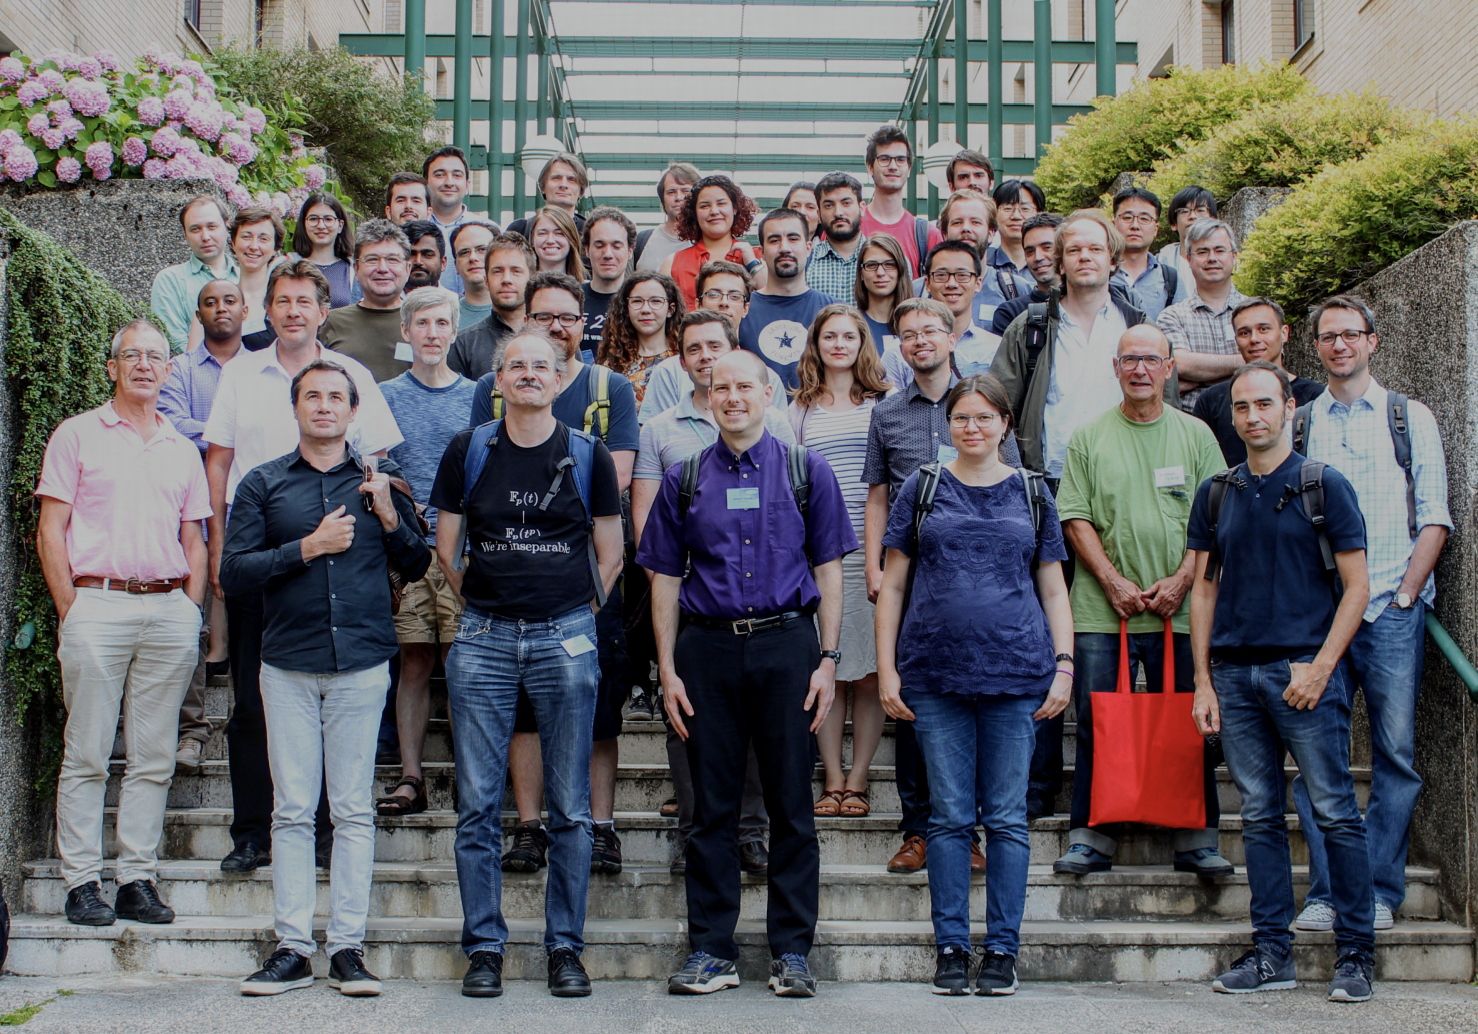
\includegraphics[width=0.90\textwidth]{images/guzvic.png}}
	\caption{\tiny Tomislav Gu{\u{z}}vi\'c}
	\end{subfigure}
	\end{figure}
\end{frame}





% Other Fields Rational EC
\begin{frame}[plain]
\begin{thm}[Gonz\'alez-Jimenez, Najman, 2016]
Let $E/\Q$ be a rational elliptic curve, and let $K/\Q$ be a number field whose smallest prime divisor is at least 7, then the only possible torsion subgroups $E(\Q)_\tors$ are those from Mazur's list, namely:
	\[
	\begin{cases}
	\Z/n\Z, & \text{with } n= 1, 2, \ldots, 10, 12 \text{ or} \\
	\Z/2\Z \oplus \Z/2n\Z, & \text{with } n= 1, 2, 3, 4
	\end{cases}
	\]
Each such possibility occurs for infinitely many elliptic curves. In fact, if the largest prime divisor is at least 11, then $E(K)_\tors=$ $E(\Q)_\tors$. 
\end{thm}
	\begin{figure}[h]
	\centering
	\begin{subfigure}{0.40\textwidth}
	\captionsetup{labelformat=empty}
	\centering
	\fbox{\includegraphics[width=0.40\textwidth]{images/jimenez2.jpeg}}
	\caption{\footnotesize \hspace{0.4cm} Enrique Gonz\'alez-Jim\'enez}
	\end{subfigure}
	%
	\begin{subfigure}{0.40\textwidth}
	\captionsetup{labelformat=empty}
	\centering
	\fbox{\includegraphics[width=0.45\textwidth]{images/najman2.png}}
	\caption{\footnotesize Filip Najman}
	\end{subfigure}
	\end{figure}
\end{frame}




% Odd Degree Galois
\begin{frame}[plain]
\ctext{Infinite Extensions of $\Q$}
\end{frame}




%%%%%%%%%%%
% Infinite Extensions 
%%%%%%%%%%%

% Maximal 2-Abelian
\begin{frame}[plain]
\footnotesize
\begin{thm}[Laska, Lorenz, 1985; Fujita, 2005]
Let $E/\Q$ be a rational elliptic curve, and let $\Q(2^\infty)$ be the maximal abelian 2-extension of $\Q$. Then $E(K)_\tors$ is isomorphic to precisely one of the following groups:
	\[
	\begin{cases}
	\Z/n\Z, & \text{with } n= 1, 3, 5, 7, 9, 15 \text{ or} \\
	\Z/2\Z \oplus \Z/2n\Z, & \text{with } n= 1, 2, 3, 4, 5, 6, 8 \text{ or} \\
	\Z/3\Z \oplus \Z/3\Z, & \text{ or} \\
	\Z/4\Z \oplus \Z/4n\Z, & \text{with } n= 1, 2, 3, 4 \text{ or} \\
	\Z/2n\Z \oplus \Z/2n\Z, & \text{with } n= 3, 4
	\end{cases}
	\]
and each such possibility occurs. 
\end{thm}
	\begin{figure}[h]
	\centering
	\begin{subfigure}{0.30\textwidth}
	\captionsetup{labelformat=empty}
	\centering
	\fbox{\includegraphics[width=0.42\textwidth]{images/laska.png}}
	\caption{\scriptsize Michael Laska}
	\end{subfigure}
	%
	\begin{subfigure}{0.30\textwidth}
	\captionsetup{labelformat=empty}
	\centering
	\fbox{\includegraphics[width=0.46\textwidth]{images/lorenz.jpeg}}
	\caption{\scriptsize Martin Lorenz}
	\end{subfigure}
	%
	\begin{subfigure}{0.30\textwidth}
	\captionsetup{labelformat=empty}
	\centering
	\fbox{\includegraphics[width=0.47\textwidth]{images/fujita.png}}
	\caption{\scriptsize Yasutsugu Fujita}
	\end{subfigure}
	\end{figure}
\end{frame}





% Maximal 3-Abelian
\begin{frame}[plain]
\footnotesize
\begin{thm}[Daniels, Lozano-Robledo, Najman, Sutherland, 2017]
Let $E/\Q$ be a rational elliptic curve. Then the torsion subgroup $E(\Q(3^\infty))_\tors$ is finite and is isomorphic to precisely one of the following groups:
	\[
	\begin{cases}
	\Z/2\Z \oplus \Z/2n\Z, & \text{with } n= 1, 2, 4, 5, 7, 8, 13 \text{ or} \\
	\Z/4\Z \oplus \Z/4n\Z, & \text{with } n= 1, 2, 4, 7 \text{ or} \\
	\Z/6\Z \oplus \Z/6n\Z, & \text{with } n= 1, 2, 3, 5, 7 \text{ or} \\
	\Z/2n\Z \oplus \Z/2n\Z, & \text{with } n= 4, 6, 7, 9. \\
	\end{cases}
	\]
All but four of the torsion subgroups, $T$, listed above occur for infinitely many $\ov{\Q}$-isomorphism classes of elliptic curves $E/\Q$. For $T \cong \Z/4\Z \oplus \Z/28\Z$, $\Z/6\Z \oplus \Z/30\Z$, $\Z/6\Z \oplus \Z/42\Z$, and $\Z/14\Z \oplus \Z/14\Z$, there are only 2, 2, 4, and 1 (respectively) $\ov{\Q}$-isomorphism classes of $E/\Q$ for which $E(\Q(3^\infty))_\tors \cong T$. 
\end{thm}
	\begin{figure}[h]
	\centering
	\begin{subfigure}{0.23\textwidth}
	\captionsetup{labelformat=empty}
	\centering
	\fbox{\includegraphics[width=0.85\textwidth]{images/daniels.jpeg}}
	\caption{\scriptsize Harris Daniels}
	\end{subfigure}
	%
	\begin{subfigure}{0.23\textwidth}
	\captionsetup{labelformat=empty}
	\centering
	\fbox{\includegraphics[width=0.72\textwidth]{images/lozano.jpeg}}
	\caption{\scriptsize \hspace{0.70cm}\'Alvaro \\ \;\;Lozano-Robledo}
	\end{subfigure}
	%
	\begin{subfigure}{0.23\textwidth}
	\captionsetup{labelformat=empty}
	\centering
	\fbox{\includegraphics[width=0.60\textwidth]{images/najman2.png}}
	\caption{\scriptsize Filip Najman}
	\end{subfigure}
	%
	\begin{subfigure}{0.23\textwidth}
	\captionsetup{labelformat=empty}
	\centering
	\fbox{\includegraphics[width=0.77\textwidth]{images/sutherland.jpg}}
	\caption{\scriptsize Andrew Sutherland}
	\end{subfigure}
	\end{figure}
\end{frame}




% D4 Extensions
\begin{frame}[plain]
\footnotesize
\begin{thm}[Daniels, 2017]
Let $E/\Q$ be a rational elliptic curve. Then $E(\Q(D_4^\infty))$ is finite and isomorphic to one of the following:
	\[
	\begin{cases}
	\Z/n\Z, & \text{with } n= 1, 3, 5, 7, 9, 13, 15 \text{ or} \\
	\Z/3\Z \oplus \Z/3n\Z, & \text{with } n= 1, 5 \text{ or} \\
	\Z/4\Z \oplus \Z/4n\Z, & \text{with } n= 1, 2, \ldots, 6, 8 \text{ or} \\
	\Z/8\Z \oplus \Z/8n\Z, & \text{with } n= 1, 2, 3, 4 \text{ or} \\
	\Z/12\Z \oplus \Z/12n\Z, & \text{with } n= 1, 2 \text{ or} \\
	\Z/n\Z \oplus \Z/n\Z, & \text{with } n= 5, 16.
	\end{cases}
	\]
All but 3 of the 24 torsion structures listed above occur for infinitely many $\overline{\Q}$-isomorphism classes of elliptic curves $E/\Q$. The torsion structures that occur finitely often are $\Z/15\Z$, $\Z/3\Z \oplus \Z/15\Z$, and $\Z/12\Z \oplus \Z/12\Z$, which occur for 4, 2, and 1 $\overline{\Q}$-isomorphism classes, respectively. 
\end{thm}
	\begin{figure}[!ht]
	\centering
	\captionsetup{labelformat=empty}
	\fbox{\includegraphics[width=0.18\textwidth]{images/daniels.jpeg}}
	\caption{\scriptsize Harris Daniels}
	\end{figure}
\end{frame}




% A4
\begin{frame}[plain]
\footnotesize
\begin{thm}[Daniels, Derickx, Hatley, 2019]
Let $E/\Q$ be an elliptic curve. The torsion subgroup $E(\Q(A_4^\infty))_\tors$ is finite and isomorphic to one of the following:
	\[
	\begin{cases}
	\Z/n\Z, & \text{with } n= 1, 3, 5, 7, 9, 13, 15, 21 \text{ or} \\
	\Z/2\Z \oplus \Z/2n\Z, & \text{with } n= 1, 2, \ldots, 9 \text{ or} \\
	\Z/3\Z \oplus \Z/3n\Z, & \text{with } n= 1, 3 \text{ or} \\
	\Z/4\Z \oplus \Z/4n\Z, & \text{with } n= 1, 2, 3, 4, 7 \text{ or} \\
	\Z/n\Z \oplus \Z/n\Z, & \text{with } n= 6, 8.
	\end{cases}
	\]
All but 4 of the 26 torsion structures listed above occur for infinitely many $\overline{\Q}$-isomorphism classes of elliptic curves $E/\Q$. The torsion structures that occur finitely often are $\Z/21\Z$, $\Z/15$, $\Z/2\Z \oplus \Z/14\Z$, and $\Z/3\Z \oplus \Z/9\Z$, which occur for 4, 2, 2, and 1 $\overline{\Q}$-isomorphism classes, respectively.  
\end{thm}
	\begin{figure}[h]
	\centering
	\begin{subfigure}{0.30\textwidth}
	\captionsetup{labelformat=empty}
	\centering
	\fbox{\includegraphics[width=0.65\textwidth]{images/daniels.jpeg}}
	\caption{\scriptsize Harris Daniels}
	\end{subfigure}
	%
	\begin{subfigure}{0.30\textwidth}
	\captionsetup{labelformat=empty}
	\centering
	\fbox{\includegraphics[width=0.52\textwidth]{images/derickx.jpg}}
	\caption{\scriptsize Maarten Derickx}
	\end{subfigure}
	%
	\begin{subfigure}{0.30\textwidth}
	\captionsetup{labelformat=empty}
	\centering
	\fbox{\includegraphics[width=0.70\textwidth]{images/hatley.png}}
	\caption{\scriptsize Jeffrey Hatley}
	\end{subfigure}
	\end{figure}
\end{frame}




% Maximal Abelian Extension
\begin{frame}[plain]
\scriptsize
\begin{thm}[Chou, 2019]
Let $E/\Q$ be a rational elliptic curve. Then $E(\Q^{\text{ab}})_\tors$ is finite, and is isomorphic to precisely one of the following groups:
	\[
	\begin{cases}
	\Z/n\Z, & \text{with } n= 1, 3, 5, 7, 9, 11, 13, 15, 17, 19, 21, 25, 27, 37, 43, 67, 163 \text{ or} \\
	\Z/2\Z \oplus \Z/2n\Z, & \text{with } n= 1, 2, \ldots, 9 \text{ or} \\
	\Z3\Z \oplus \Z/3n\Z, & \text{with } n= 1, 3 \text{ or} \\
	\Z/4\Z \oplus \Z/4n\Z, & \text{with } n= 1, 2, 3, 4 \text{ or} \\
	\Z/n\Z \oplus \Z/n\Z, & \text{with } n= 5, 6, 8.
	\end{cases}
	\]
Each of the listed groups appears as a torsion subgroup for $E(\Q^{\text{ab}})_\tors$ for some elliptic curve over $\Q$. 
\end{thm}
	\begin{figure}[!ht]
	\centering
	\captionsetup{labelformat=empty}
	\fbox{\includegraphics[width=0.20\textwidth]{images/chou.jpg}}
	\caption{Michael Chou}
	\end{figure}
\end{frame}





% Zp Extensions
\begin{frame}[plain]
\footnotesize
\begin{thm}[Chou, Daniels, Krijan, Najman, 2018]
Let $p$ be a prime, and let $E/\Q$ be an elliptic curve. Then if $p= 2, 3$, then $E(\Q_{\infty, p})_\tors$ is one of the following groups:
	\[
	\begin{cases}
	\Z/n\Z, & n= 1, 2, \ldots, 10, 12, 21^*, 27^* \text{ or} \\
	\Z/2\Z \oplus \Z/2n\Z, & n= 1, 2, 3, 4, \\
	\end{cases}
	\]
where the starred cases can only occur if $p= 3$. If $p \neq 2, 3$, then $E(\Q_{\infty, p})_\tors=$ $E(\Q)_\tors$. Each of the groups listed above appears as a torsion subgroup for $E(\Q_{\infty,p})_\tors$ for some $E/\Q$ and each $p$ possible.
\end{thm}

	\begin{figure}[h]
	\centering
	\begin{subfigure}{0.23\textwidth}
	\captionsetup{labelformat=empty}
	\centering
	\fbox{\includegraphics[width=0.64\textwidth]{images/chou.jpg}}
	\caption{\scriptsize Michael Chou}
	\end{subfigure}
	%
	\begin{subfigure}{0.23\textwidth}
	\captionsetup{labelformat=empty}
	\centering
	\fbox{\includegraphics[width=0.85\textwidth]{images/daniels.jpeg}}
	\caption{\scriptsize Harris Daniels}
	\end{subfigure}
	%
	\begin{subfigure}{0.23\textwidth}
	\captionsetup{labelformat=empty}
	\centering
	\fbox{\includegraphics[width=0.64\textwidth]{images/krijan.jpeg}}
	\caption{\scriptsize Ivan Krijan}
	\end{subfigure}
	%
	\begin{subfigure}{0.23\textwidth}
	\captionsetup{labelformat=empty}
	\centering
	\fbox{\includegraphics[width=0.60\textwidth]{images/najman2.png}}
	\caption{\scriptsize Filip Najman}
	\end{subfigure}
	\end{figure}
\end{frame}





% Zp Other
\begin{frame}[plain]
\scriptsize
\begin{thm}[Gu{\u{z}}vi\'c, Vukorepa, 2022]
Let $E/\Q$ be an elliptic curve. Then $E(\Q(\zeta_{16}))_\tors \in \Phi(1)$ or is one of $\Z/4\Z \oplus \Z/4\Z$, $\Z/2\Z \oplus \Z/10\Z$ and $E(\Q(\zeta_{27}))_\tors \in \Phi(1)$ or is one of $\Z/3\Z \oplus \Z/3n\Z$ with $n= 1, 2, 3$, $\Z/21\Z$, or $\Z/27\Z$. Furthermore, let $p \in \{5, 7, 11 \}$. Then either $E(\Q(\zeta_p))_\tors \in \Phi(1)$ or is one of $\Z/5\Z \oplus \Z/5\Z$, $\Z/15\Z$, or $\Z/16\Z$, if $p= 5$, or $\Z/n\Z$ with $n= 13, 14, 18$ or $\Z/2\Z \oplus \Z/2n\Z$ with $n= 7, 9$, if $p= 7$, or $\Z/11\Z$, $\Z/25\Z$, or $\Z/2\Z \oplus \Z/10\Z$, if $p= 11$. 
\end{thm}

\begin{thm}[Gu{\u{z}}vi\'c, Krijan, 2020]
Let $\mathcal{K}= \prod_{p \text{ prime}} \Q_{\infty, p}$ and $\mathcal{K}_{\geq p}= \prod_{q \text{ prime}, q \geq p}$, and let $E/\Q$ be an elliptic curve. Then $E(\mathcal{K}_{\geq 5})_\tors= E(\Q)_\tors$ and $E(\mathcal{K})_\tors$ is isomorphic to precisely one of the following:
	\[
	\begin{cases}
	\Z/n\Z, & \text{with } n= 1, 2, \ldots, 10, 12, 13, 21, 27 \text{ or} \\
	\Z/2\Z \oplus \Z/2n\Z, & \text{with } n= 1, 2, 3, 4. \\
	\end{cases}
	\]
Moreover, each such group above occurs for some elliptic curve $E/\Q$. 
\end{thm}

	\begin{figure}[h]
	\centering
	\begin{subfigure}{0.23\textwidth}
	\captionsetup{labelformat=empty}
	\centering
	\fbox{\includegraphics[width=0.72\textwidth]{images/guzvic2.jpg}}
	\caption{\scriptsize Tomislav Gu{\u{z}}vi\'c}
	\end{subfigure}
	%
	\begin{subfigure}{0.23\textwidth}
	\captionsetup{labelformat=empty}
	\centering
	\fbox{\includegraphics[width=0.65\textwidth]{images/krijan.jpeg}}
	\caption{\scriptsize Ivan Krijan}
	\end{subfigure}
	%
	\begin{subfigure}{0.30\textwidth}
	\captionsetup{labelformat=empty}
	\centering
	\fbox{\includegraphics[width=0.50\textwidth]{images/vukorepa.jpeg}}
	\caption{\scriptsize Borna Vukorepa}
	\end{subfigure}
	\end{figure}
\end{frame}





% Odd Degree Galois
\begin{frame}[plain]
\ctext{Classification over Odd Degree Galois Fields}
\end{frame}



% Quartic Galois Rational EC
\begin{frame}[plain]
\small
\begin{thm}[Chou, 2015]
Let $E/\Q$ be a rational elliptic curve, and let $K/\Q$ be a quartic Galois number field. Then the possible torsion subgroups $E(K)_\tors$ are precisely:
	\[
	\begin{cases}
	\Z/n\Z, & \text{with } n= 1, 2, \ldots, 10, 12, 13, 15, 16 \text{ or} \\
	\Z/2\Z \oplus \Z/2n\Z, & \text{with } n= 1, 2, \ldots, 6, 8 \text{ or} \\
	\Z/3\Z \oplus \Z/3n\Z, & \text{with } n= 1, 2 \text{ or} \\
	\Z/4\Z \oplus \Z/4n\Z, & \text{with } n= 1, 2 \text{ or} \\
	\Z/5\Z \oplus \Z/5\Z, & \text{or} \\
	\Z/6\Z \oplus \Z/6\Z.
	\end{cases}
	\]
\end{thm}
	\begin{figure}[!ht]
	\centering
	\captionsetup{labelformat=empty}
	\fbox{\includegraphics[width=0.20\textwidth]{images/chou.jpg}}
	\caption{Michael Chou}
	\end{figure}
\end{frame}








%%%%%%%%%%%
% Nonic Galois Classification
%%%%%%%%%%%

% Nonic Galois Classification
\begin{frame}[plain]
\ctext{Nonic Galois Classification}
\end{frame}



% Outline
\begin{frame}[plain]
\frametitle{Outline of the Classification}
        \begin{enumerate}
        \item Determine the possible prime orders. \vfill
        \item Bound the $p$-Sylow Subgroups. \vfill
        \item Create a finite list of possibilities. \vfill
        \item Find examples and eliminate cases. \vfill
        \end{enumerate}
\vfill
\end{frame}





% Step 1. Determine the Possible Prime Orders
\begin{frame}[plain]
\vfill
\begin{center} {\bfseries \Large \textcolor{UniOrange}{Step 1. Determine the Possible Prime Orders}} \end{center}
\vfill 
\end{frame}





% Lozano-Robledo S(d)
\begin{frame}[plain,c]
\begin{thm}[Lozano-Robledo, 2013]
Let $S_\Q(d)$ be the set of primes such that there exists an elliptic curve $E/\Q$ with a point of order $p$ defined in an extension $K/\Q$ of degree at most $d$. Then $S_\Q(9)= \{ 2, 3, 5, 7, 11, 13, 17, 19 \}$.
\end{thm}

	\begin{figure}[h]
	\centering
	\begin{subfigure}{\textwidth}
	\captionsetup{labelformat=empty}
	\centering
	\fbox{\includegraphics[width=0.2\textwidth]{images/robledo.jpg}}
	\caption{\'Alvaro Lozano-Robledo}
	\end{subfigure}
	\end{figure}
\end{frame}





% Gonzalez-Jimenez, Najman R(d)
\begin{frame}[plain,c]
\begin{prop}[Gonz\'alez-Jim\'enez, Najman, 2016] \hfill
	\begin{enumerate}[(i)]
	\item $11 \in R_\Q(d)$ if and only if $5 \mid d$.
	\item $17 \in R_\Q(d)$ if and only if $8 \mid d$.
	\end{enumerate}
\end{prop}
	\begin{figure}[h]
	\centering
	\begin{subfigure}{0.35\textwidth}
	\captionsetup{labelformat=empty}
	\centering
	\fbox{\includegraphics[width=0.45\textwidth]{images/jimenez.png}}
	\caption{Enrique Gonz\'alez-Jim\'enez}
	\end{subfigure}
	%
	\begin{subfigure}{0.3\textwidth}
	\captionsetup{labelformat=empty}
	\centering
	\fbox{\includegraphics[width=0.50\textwidth]{images/najman2.png}}
	\caption{Filip Najman}
	\end{subfigure}
	\end{figure}

\begin{lem} \small
Let $E/\Q$ be a rational elliptic curve, and let $K/\Q$ be a nonic Galois field. If $P \in E(K)$ is a point of prime order $p$, then $p \in \{ 2, 3, 5, 7, 13,$ $19 \}$.
\end{lem}
\end{frame}






% Step 2. Bound the Size of the Sylow Subgroups
\begin{frame}[plain]
\vfill
\begin{center} {\bfseries \Large \textcolor{UniOrange}{Step 2. Bound the Size of the Sylow Subgroups}} \end{center}
\vfill 
\end{frame}


% Full 2-Torsion, Lozano-Robledo
\begin{frame}[plain]
\begin{thm}[Gonz\'alez-Jim\'enez, Lozano-Robledo]
Let $E/\Q$ be an elliptic curve without CM. Let $1 \leq s \leq N$ be fixed integers, and let $T \subseteq E[2^N]$ be a subgroup isomorphic to $\Z/2^s/Z \oplus \Z/2^N \Z$. Then $[\Q(T) \colon \Q]$ is divisible by 2 if $s=N=2$, and otherwise by $2^{2N+2s-8}$ if $N \geq 3$, unless $s \geq 4$ and $j(E)$ is one of the two values:
	\[
	- \dfrac{3 \cdot 18249920^3}{17^{16}}\; \text{ or } - \dfrac{7 \cdot 1723187806080^3}{79^{16}}
	\]
in which case $[\Q(T) \colon \Q]$ is divisible by $3 \cdot 2^{2N+2s-9}$. Moreover, this is best possible in that there are one-parameter families $E_{s,N}(t)$ of elliptic curves over $\Q$ such that for each $s, N \geq 0$ and each $t \in \Q$, and subgroups $T_{s,N} \in E_{s,N}(t)(\ov{\Q})$ isomorphic to $\Z/2^s\Z \oplus \Z/2^N\Z$ such that $[\Q(T_{s,N}) \colon \Q]$ is equal to the bound given above. 
\end{thm}

\begin{lem}[Najman, 2015] \small
If $E(\Q)$ has a nontrivial 2-Sylow subgroup, then $E(K)[2^\infty]= E(\Q)[2^\infty]$. 
\end{lem}
\end{frame}



% 2-Sylow Bound
\begin{frame}[plain,c]
\begin{lem}[M.]
Let $E/\Q$ be a rational elliptic curve, and let $K/\Q$ be a nonic Galois field. Then $E(K)[2^\infty] \subseteq \Z/2\Z \oplus \Z/8\Z$.
\end{lem}
\end{frame}



% Full p-Torsion & Weil-Pairing
\begin{frame}[plain,c]
\begin{lem}[Odd Torsion]
Let $K/\Q$ be an odd degree number field, and let $E/\Q$ be a rational elliptic curve. Then $E(K)_\tors$ does not contain full $p$-torsion for all odd primes.
\end{lem}

\begin{lem}[Galois Isogeny]
Let $K/\Q$ be a Galois extension, and let $E/\Q$ be a rational elliptic curve. If $E(K)[n] \cong \Z/n\Z$, then $E$ has a rational $n$-isogeny. Furthermore, if $(K)_\tors \cong \Z/m\Z \oplus \Z/mn\Z$, then $E$ has a rational $n$-isogeny. 
\end{lem}
\end{frame}





% Q-Isogeny Classification
\begin{frame}[plain]
\footnotesize
\begin{thm}[Fricke, Kenku, Klein, Kubert, Ligozat, Mazur, Ogg, et al.]
Let $N \geq 2$ be such that $X_0(N)$ has a non-cuspidal $\Q$-rational point. Then
	\begin{enumerate}[(i)]
	\item $N \leq 10$ or $N=$ 12, 13, 16, 18, or 25. In this case, $X_0(N)$ is a curve of genus 0, and the $\Q$ rational points on $X_0(N)$ form an infinite 1-parameter family, or
	\item $N=$ 11, 14, 15, 17, 19, 21, or 27, i.e. $X_0(N)$ is a rational elliptic curve (in each case $X_0(N)(\Q)$ is finite, or
	\item $N=$ 37, 43, 67, or 163. In this case, $X_0(N)$ is a curve of genus $\geq 2$ and by Faltings' Theorem has only finitely many $\Q$-rational points. 
	\end{enumerate}
In particular, a rational elliptic curve may only have a rational cyclic $n$-isogeny for $n \leq 19$ or $n \in \{ 21, 25, 27, 37, 43, 67,163\}$. Furthermore, if $E$ does not have CM, then $n \leq 18$ or $n \in \{ 21, 25, 37 \}$.
\end{thm}
\end{frame}





% Sylow Bound, p > 2
\begin{frame}[plain,c]

\begin{lem}[M.]
Let $E/\Q$ be a rational elliptic curve, and let $K/\Q$ be a nonic Galois field. Then
	\[
	\begin{aligned}
	E(K)[3^\infty]&\subseteq \Z/27\Z \\
	E(K)[5^\infty]&\subseteq \Z/25\Z \\
	E(K)[7^\infty]&\subseteq \Z/7\Z \\
	E(K)[13^\infty]&\subseteq \Z/13\Z \\
	E(K)[19^\infty]&\subseteq \Z/19\Z
	\end{aligned}
	\]
\end{lem}
\end{frame}





% Step 3. Create a Finite List of Possibilities
\begin{frame}[plain]
\vfill
\begin{center} {\bfseries \Large \textcolor{UniOrange}{Step 3. Create a Finite List of Possibilities}} \end{center}
\vfill 
\end{frame}





% Finite List
\begin{frame}[plain,c]
\footnotesize
\begin{lem}[M.]
Let $E/\Q$ be a rational elliptic curve, and let $K/\Q$ be a nonic Galois field. Then $E(K)_\tors$ is isomorphic to one of the following (although not all cases need occur):
	\[
	\begin{cases}
	\Z/n\Z, & n= 1, 2, \ldots, 10, 12, 13, 14, 15, 18, 19, 21, 25, 27 \\
	\Z/2\Z \oplus \Z/2n\Z, & n= 1, 2, \ldots, 7, 9, 10, 12, 13, 14, 15, 18, 19, 21, 25, 27
	\end{cases}
	\]
\end{lem}
\end{frame}





% Step 4. Find Examples \& Eliminate Cases
\begin{frame}[plain]
\vfill
\begin{center} {\bfseries \Large \textcolor{UniOrange}{Step 4. Find Examples \& Eliminate Cases}} \end{center}
\vfill 
\end{frame}





% Base Extension
\begin{frame}[plain,c]

\ctext{I. Base Extension}

\begin{lem}[M.]
Let $E/\Q$ be a rational elliptic curve, and let $F/\Q$ be a cubic Galois field. Then there exists a nonic Galois field $K$ such that $E(K)_\tors \cong E(F)_\tors$. Hence, $\Phi_\Q^{\Gal}(3) \subseteq \Phi_\Q^{\Gal}(9)$.
\end{lem}
\end{frame}





% Examples of Torsion Subgroups
\begin{frame}[plain,c]
	\begin{table}[!ht]
	\centering
	\caption{Examples of torsion subgroups $\Phi_\Q(3) \setminus \Phi(1)$.\label{tab:3qsm1}}
	\begin{tabular}{ccc} \hline
	Torsion Subgroup & Elliptic Curve & Galois Cubic Field \\ \hline
	$\Z/13\Z$ & \ofsbo{} & \qzetasp{} \\
	$\Z/14\Z$ & \fnat{} & \qzetasp{} \\
	$\Z/18\Z$ & \ofaf{} & \qzetasp{} \\
	$\Z/21\Z$ & \ostbo{} & \qzetanp{} \\
	$\Z/2\Z \times \Z/14\Z$ & \onttco{} & \ttnsoo{}
	\end{tabular}
	\end{table}

        \begin{table}[!ht]
        \centering
        \caption{Examples of $E(K)$ with 19 and 27-torsion over nonic fields.\label{tab:1927tor}}
        \begin{tabular}{cccc} \hline
        $E(K)_\tors$ & $E(\Q)_\tors$ &  $E$ & $K$ \\ \hline
        $\Z/19\Z$ & $\{ \O \}$ & \tsoao{} & \qzetantp{} \\ 
        $\Z/27\Z$ & $\Z/3\Z$ & \tsaf{} & \qzetatsp{}
        \end{tabular}
        \end{table}
\end{frame}





% Remaining Groups
\begin{frame}[plain,c]
This leaves the following list of torsion subgroups whose existence or non-existence we have yet to prove. 
	\[
	\begin{cases}
	\Z/n\Z, & n= 15, 25 \\
	\Z/2\Z \oplus \Z/2n\Z, & n= 5, 6, 9, 10, 12, 13, 14, 15, 18, 19, 21, 25, 27
	\end{cases}
	\]
\end{frame}





% Najman Growth Lemmas
\begin{frame}[plain,c]
\begin{lem}[Najman, 2015]
Let $p, q$ be distinct odd primes, $F_2/F_1$ a Galois extension of number fields such that $\Gal(F_2/F_1) \simeq \Z/q\Z$ and $E/F_1$ an elliptic curve with no $p$-torsion over $F_1$. Then if $q$ does not divide $p-1$ and $\Q(\zeta_p) \not\subset F_2$, then $E(F_2)[p]=0$. 
\end{lem}


\begin{lem}[Najman, 2015]
Let $p$ be an odd prime number, $q$ a prime not dividing $p$, $F_2/F_1$ a Galois extension of number fields such that $\Gal(F_2/F_1) \simeq \Z/q\Z$, $E/F_1$ an elliptic curve, and suppose $E(F_1) \supset \Z/p\Z$, $E(F_1) \not\supset \Z/p^2\Z$, and $\zeta_p \notin F_2$. Then $E(F_2) \not\supset \Z/p^2\Z$.
\end{lem} 
\end{frame}





% E(K)[5^\infty]= E(\Q)[5^\infty]
\begin{frame}[plain,c]

\begin{lem}[Najman, 2015]
Let $K$ be a cubic field and let $E/\Q$ be a rational elliptic curve. Then the 5-Sylow groups of $E(\Q)$ and $E(K)$ are equal. 
\end{lem}

\begin{lem}[M.]
Let $E/\Q$ be a rational elliptic curve, and let $K/\Q$ be a nonic Galois field. Then the 5-Sylow subgroup of $E(\Q)_\tors$ and $E(K)_\tors$ are equal, i.e. $E(\Q)[5^\infty]= E(K)[5^\infty]$.
\end{lem}

\end{frame}





% Z/2Z x Z/10Z
\begin{frame}[plain,c]
\footnotesize
\begin{lem}[M.]
Let $E/\Q$ be a rational elliptic curve, and let $K/\Q$ be a nonic Galois field. Then $E(K)_\tors$ does not contain $\Z/2\Z \oplus \Z/10\Z$.
\end{lem} \pspace

\pfsk
\begin{itemize}
\item By our previous result, we know that $E(K)[5^\infty]= E(\Q)[5^\infty] \cong \Z/5\Z$. 
\item Choosing a model $E: y^2= x^3 + Ax + B$, we know the $x$-coordinates of points of order 2 correspond to roots of $x^3 + Ax + B$. 
\item As $E(K)_\tors \supseteq \Z/2\Z \oplus \Z/2\Z$, $K$ contains a splitting field for $x^3 + Ax + B$, which has degree 1, 3, or 6. 
\item Degree 6 is not possible as $K/\Q$ has odd degree. Then $\Q(E(K)[2^\infty])$ is defined over at most a cubic field. 
\item But then either $E(\Q)_\tors \cong \Z/2\Z \oplus \Z/10\Z$ or there is a cubic field, $F$, with $E(F)_\tors \cong \Z/2\Z \oplus \Z/10\Z$, contradicting the classification of either $\Phi(1)$ or $\Phi_\Q(3)$. \hfill\qed
\end{itemize}
\end{frame}





% Field of Definition Degree
\begin{frame}[plain,c]
\begin{lem}[M.]
Let $E/\Q$ be a rational elliptic curve, and let $K/\Q$ be a nonic Galois field. Suppose $P \in E(K)_\tors$ is a point of order $p$. Then
        \begin{enumerate}[(i)]
        \item if $p \in \{ 3, 5 \}$, then $P$ is defined over $\Q$, i.e. $P \in E(\Q)[p]$.
        \item if $p= 13$, then there is a cubic field $F \subseteq K$ with $P \in E(F)[p]$. 
        \item if $p \in \{ 2, 7 \}$, then $P$ is defined over $\Q$, i.e. $P \in E(\Q)[p]$, or there is a cubic field $F \subseteq K$ with $P \in E(F)[p]$. 
        \end{enumerate}
\end{lem}
\end{frame}





% (15), (2, 26), (2,42), (2,18)
\begin{frame}[plain,c]
\footnotesize

\begin{lem}[M.]
Let $E/\Q$ be a rational elliptic curve, and let $K/\Q$ be a nonic Galois field. Then $E(K)_\tors$ is not isomorphic to $\Z/15\Z$, $\Z/2\Z \oplus \Z/26\Z$, or $\Z/2\Z \oplus \Z/42\Z$. 
\end{lem}

\begin{lem}[M.]
Let $E/\Q$ be a rational elliptic curve, and let $K/\Q$ be an odd degree Galois field. Then $E(K)_\tors$ does not contain a subgroup isomorphic to $\Z/2\Z \oplus \Z/18\Z$. 
\end{lem}

\pfsk 
\begin{itemize} 
\item As $\Z/9\Z \subseteq E(K)_\tors$, we know that $E$ has a rational 9-isogeny. But then $E$ is a twist of an elliptic curve with $j$-invariant given by
	\[
	j= \dfrac{h^3(h^3 - 24)^3}{h^3 - 27}
	\]
\item From a result of Kubert, there are no rational elliptic curves with a rational 9-isogeny and full 2-torsion. Then $E(\Q)_\tors= \{ \O \}$. 
\item Choose a model $E: y^2= x^3 + Ax + B$. We know $E(K)_\tors \supseteq \Z/2\Z \oplus \Z/2\Z$ so that $K$ contains a splitting field for $x^3 + Ax + B$, say $F$. \item As $F/\Q$ is Galois, $\disc( x^3 + Ax + B)$ is a square. 
\item Giving the discriminant in terms of $h$ and ``absorbing squares'', this implies a rational solution $(m, n)$ to $m^2= n^3 - 27$. This is an elliptic curve with $E(\Q)= \{ \O, (3,0) \}$. The point $(3, 0)$ corresponds to a cusp. Therefore, $E(K)_\tors \not\supseteq \Z/2\Z \oplus \Z/18\Z$. \hfill\qed
\end{itemize}
\end{frame}





% Z/2Z x Z/12Z
\begin{frame}[plain,c]
\footnotesize
\begin{lem}[Najman, 2015]
Let $E/\Q$ be a rational elliptic curve, and let $K/\Q$ be a cubic Galois field. If $E(\Q)$ has no points of order 4, then $E(K)$ has no 4-torsion. 
\end{lem}

\begin{lem}[M.]
Let $E/\Q$ be a rational elliptic curve, and let $K/\Q$ be a nonic Galois field. Then $E(K)_\tors$ does not contain $\Z/2\Z \oplus \Z/12\Z$.
\end{lem}

\pfsk Either $E(\Q)[2^\infty] \not\cong \{ \O \}$ or not.
	\begin{enumerate}[(i)] \footnotesize
	\item $E(\Q)[2^\infty] \not\cong \{ \O \}$: Then $E(K)[2^\infty]= E(\Q)[2^\infty] \cong \Z/2\Z \oplus \Z/4\Z$. We know the point of order 3 is defined over $\Q$. But then $E(\Q)_\tors \cong \Z/2\Z \oplus \Z/12\Z$, contradicting the classification of $\Phi(1)$. 
	\item $E(\Q)[2^\infty]= \{ \O \}$: Let $F$ be a cubic subfield of $K$. Because $E(\Q)$ has no points of order 4, we know by Najman's Lemma that $E(F)$ has no points of order 4. Then the point of order 4 is strictly defined over a nonic field.\pspace
	
	Choose a model $E: y^2= x^3 + Ax + B$. If $P= (x(P), y(P))$ is a point of order 4 on $E$, then $x(P)$ is a root for 
		\[
		\Psi_4(x)= 4( x^6 + 5Ax^4 + 20Bx^3 - 5A^2x^2 - 4ABx - 8B^2 - A^3)
		\]
	This contradicts the fact that $x$ was defined over a nonic field. \hfill \qed
	\end{enumerate}
\end{frame}





% Nonic Galois Result
\begin{frame}[plain,c]
\begin{thm}[M.]
Let $E/\Q$ be a rational elliptic curve, and let $K/\Q$ be a nonic Galois field. Then $E(K)_\tors$ is isomorphic to precisely one of the following:
	\[
	\begin{cases}
	\Z/n\Z, & n= 1, 2, \ldots, 10, 12, 13, 14, 18, 19, 21, 27 \\
	\Z/2\Z \oplus \Z/2n\Z, & n= 1, 2, 3, 4, 7
	\end{cases}
	\]
\end{thm}
\end{frame}





% Nonic Galois Examples
\begin{frame}[plain,c]
	\begin{table}[!ht]
	\centering
	\caption{Examples of each possible $E(K)_\tors$ in $\Phi_\Q^{\Gal}(9)$.}
	\resizebox{!}{0.36\textwidth}{%
	\begin{tabular}{cccc} \hline
	 $E(K)_\tors$ & Cremona Label & $E(\Q)_\tors$ & $K$ \\ \hline
	$\{ \O \}$ & \ooat{} & $\{ \O \}$ & \qzetantp{} \\
	$\Z/2\Z$ & \ffafiv{} & $\Z/2\Z$ & \qzetantp{} \\
	$\Z/3\Z$ & \onao{} & $\Z/3\Z$ & \qzetantp{} \\
	$\Z/4\Z$ & \ofas{} & $\Z/4\Z$ & \qzetantp{} \\
	$\Z/5\Z$ & \ooao{} & $\Z/5\Z$ & \qzetantp{} \\
	$\Z/6\Z$ & \ofat{} & $\Z/6\Z$ & \qzetantp{} \\
	$\Z/7\Z$ & \tsbo{} & $\Z/7\Z$ & \qzetantp{} \\
	$\Z/8\Z$ & \ffafo{} & $\Z/8\Z$ & \qzetantp{} \\
	$\Z/9\Z$ & \ffbt{} & $\Z/9\Z$ & \qzetantp{} \\
	$\Z/10\Z$ & \ssco{} & $\Z/10\Z$ & \qzetantp{} \\
	$\Z/12\Z$ & \nzct{} & $\Z/12\Z$ & \qzetantp{} \\
	$\Z/13\Z$ & \ofsbo{} & $\{ \O \}$ & \qzetantp{} \\
	$\Z/14\Z$ & \fnaf{} & $\Z/2\Z$ & \qzetantp{} \\
	$\Z/18\Z$ & \tszsozot{} & $\Z/6\Z$ & \nnezsb{} \\
	$\Z/19\Z$ & \tsoao{} & $\{ \O \}$ & \qzetantp{} \\
	$\Z/21\Z$ & \ostbo{} & $\Z/3\Z$ & \nnstfttf{} \\
	$\Z/27\Z$ & \tsaf{} & $\Z/3\Z$ & \qzetatsp{} \\
	$\Z/2\Z \oplus \Z/2\Z$ & \ffat{} & $\Z/2\Z \oplus \Z/2\Z$ & \qzetantp{} \\
	$\Z/2\Z \oplus \Z/4\Z$ & \ffao{} & $\Z/2\Z \oplus \Z/4\Z$ & \qzetantp{} \\
	$\Z/2\Z \oplus \Z/6\Z$ & \tzat{} & $\Z/2\Z \oplus \Z/6\Z$ & \qzetantp{} \\
	$\Z/2\Z \oplus \Z/8\Z$ & \tozet{} & $\Z/2\Z \oplus \Z/8\Z$ & \qzetantp{} \\
	$\Z/2\Z \oplus \Z/14\Z$ & \onttco{} & $\{ \O \}$ & \nnstfttfz{} \\
	\end{tabular}
	}
	\end{table}
\end{frame}








% By Galois Type
\begin{frame}[plain,c]
\begin{thm}[M.]
Let $E/\Q$ be a rational elliptic curve, and let $K/\Q$ be a nonic bicyclic Galois field, i.e. a nonic field with $\Gal(K/\Q) \cong \Z/3\Z \oplus \Z/3\Z$. Then $E(K)_\tors$ is precisely one of the following:
	\[
	\begin{cases}
	\Z/n\Z, & n= 1, 2, \ldots, 10, 12, 13, 14, 18, 21 \\
	\Z/2\Z \oplus \Z/2n\Z, & n= 1, 2, 3, 4, 7
	\end{cases}
	\]
\end{thm}
\begin{thm}[M.]
Let $E/\Q$ be a rational elliptic curve, and let $K/\Q$ be a nonic cyclic Galois field, i.e. a nonic field with $\Gal(K/\Q) \cong \Z/9\Z$. Then $E(K)_\tors$ is precisely one of the following:
	\[
	\begin{cases}
	\Z/n\Z, & n= 1, 2, \ldots, 10, 12, 13, 14, 21 \\
	\Z/2\Z \oplus \Z/2n\Z, & n= 1, 2, 3, 4
	\end{cases}
	\]
\end{thm}
\end{frame}





% Bicyclic Examples
\begin{frame}[plain,c]
	\begin{table}[!ht] 
	\centering
	\caption{Examples of torsion subgroups $E(K)_\tors$ in $\Phi_\Q^{\cC_3 \times \cC_3}(9)$.}
	\resizebox{!}{0.36\textwidth}{%
	\begin{tabular}{cccc} \hline
	 $E(K)_\tors$ & Cremona Label & $E(\Q)_\tors$ & $K$ \\ \hline
	$\{ \O \}$ & \ooat{} & $\{ \O \}$ & \nnstfttf{} \\
	$\Z/2\Z$ & \ffafiv{} & $\Z/2\Z$ & \nnstfttf{} \\
	$\Z/3\Z$ & \onao{} & $\Z/3\Z$ & \nnstfttf{} \\
	$\Z/4\Z$ & \ofas{} & $\Z/4\Z$ & \nnstfttf{} \\
	$\Z/5\Z$ & \ooao{} & $\Z/5\Z$ & \nnstfttf{} \\
	$\Z/6\Z$ & \ofat{} & $\Z/6\Z$ & \nnstfttf{} \\
	$\Z/7\Z$ & \tsbo{} & $\Z/7\Z$ & \nnstfttf{} \\
	$\Z/8\Z$ & \ffaf{} & $\Z/8\Z$ & \nnstfttf{} \\
	$\Z/9\Z$ & \ffbt{} & $\Z/9\Z$ & \nnstfttf{} \\
	$\Z/10\Z$ & \ssco{} & $\Z/10\Z$ & \nnstfttf{} \\
	$\Z/12\Z$ & \nzct{} & $\Z/12\Z$ & \nnstfttf{} \\
	$\Z/13\Z$ & \ofsbo{} & $\{ \O \}$ & \nnstfttf{} \\
	$\Z/14\Z$ & \fnaf{} & $\Z/2\Z$ & \nnstfttf{} \\
	$\Z/18\Z$ & \ofaf{} & $\Z/6\Z$ & \nnstfttf{} \\
	$\Z/21\Z$ & \ostbo{} & $\Z/3\Z$ & \qzetatsp{} \\
	$\Z/2\Z \oplus \Z/2\Z$ & \ffat{} & $\Z/2\Z \oplus \Z/2\Z$ & \nnstfttf{} \\
	$\Z/2\Z \oplus \Z/4\Z$ & \ffao{} & $\Z/2\Z \oplus \Z/4\Z$ & \nnstfttf{} \\
	$\Z/2\Z \oplus \Z/6\Z$ & \tzat{} & $\Z/2\Z \oplus \Z/6\Z$ & \nnstfttf{} \\
	$\Z/2\Z \oplus \Z/8\Z$ & \tozet{} & $\Z/2\Z \oplus \Z/8\Z$ & \nnstfttf{} \\
	$\Z/2\Z \oplus \Z/14\Z$ & \onttco{} & $\{ \O \}$ & \nnstfttfz{} \\
	\end{tabular}
	}
	\end{table}
\end{frame}



% Cyclic Nonic Examples
\begin{frame}[plain,c]
	\begin{table}[!ht] 
	\centering
	\caption{Examples of torsion subgroups $E(K)_\tors$ in $\Phi_\Q^{\cC_9}(9)$.}
	\resizebox{!}{0.36\textwidth}{%
	\begin{tabular}{cccc} \hline
	 $E(K)_\tors$ & Cremona Label & $E(\Q)_\tors$ & $K$ \\ \hline
	$\{ \O \}$ & \ooat{} & $\{ \O \}$ & \qzetantp{} \\
	$\Z/2\Z$ & \ffafiv{} & $\Z/2\Z$ & \qzetantp{} \\
	$\Z/3\Z$ & \onao{} & $\Z/3\Z$ & \qzetantp{} \\
	$\Z/4\Z$ & \ofas{} & $\Z/4\Z$ & \qzetantp{} \\
	$\Z/5\Z$ & \ooao{} & $\Z/5\Z$ & \qzetantp{} \\
	$\Z/6\Z$ & \ofat{} & $\Z/6\Z$ & \qzetantp{} \\
	$\Z/7\Z$ & \tsbo{} & $\Z/7\Z$ & \qzetantp{} \\
	$\Z/8\Z$ & \ffaf{} & $\Z/8\Z$ & \qzetantp{} \\
	$\Z/9\Z$ & \ffbt{} & $\Z/9\Z$ & \qzetantp{} \\
	$\Z/10\Z$ & \ssco{} & $\Z/10\Z$ & \qzetantp{} \\
	$\Z/12\Z$ & \nzct{} & $\Z/12\Z$ & \qzetantp{} \\
	$\Z/13\Z$ & \ofsbo{} & $\{ \O \}$ & \qzetantp{} \\
	$\Z/18\Z$ & \tszsozot{} & $\Z/6\Z$ & \nnezsb{} \\
	$\Z/21\Z$ & \ostbo{} & $\Z/3\Z$ & \nnstfttf{} \\
	$\Z/27\Z$ & \tsaf{} & $\Z/3\Z$ & \qzetatsp{} \\
	$\Z/2\Z \oplus \Z/2\Z$ & \ffat{} & $\Z/2\Z \oplus \Z/2\Z$ & \qzetantp{} \\
	$\Z/2\Z \oplus \Z/4\Z$ & \ffao{} & $\Z/2\Z \oplus \Z/4\Z$ & \qzetantp{} \\
	$\Z/2\Z \oplus \Z/6\Z$ & \tzat{} & $\Z/2\Z \oplus \Z/6\Z$ & \qzetantp{} \\
	$\Z/2\Z \oplus \Z/8\Z$ & \tozet{} & $\Z/2\Z \oplus \Z/8\Z$ & \qzetantp{} \\
	\end{tabular}
	}
	\end{table}
\end{frame}



% Torsion Growth Result 
\begin{frame}[plain,c]
\begin{table}[]
\centering
\resizebox{!}{0.33\textwidth}{%
\begin{tabular}{|l|c|c|c|c|c|c|c|c|c|c|c|c|c|c|c|} \hline
\diagbox[width=6.8em]{$E(K)_\tors$}{$E(\Q)_\tors$}
 & $\mathcal{C}_1$ & $\mathcal{C}_2$ & $\mathcal{C}_3$ & $\mathcal{C}_4$ & $\mathcal{C}_5$ & $\mathcal{C}_6$ & $\mathcal{C}_7$ & $\mathcal{C}_8$ & $\mathcal{C}_9$ & $\mathcal{C}_{10}$ & $\mathcal{C}_{12}$ & $\mathcal{C}_2 \times \mathcal{C}_2$ & $\mathcal{C}_2 \times \mathcal{C}_4$ & $\mathcal{C}_2 \times \mathcal{C}_6$ & $\mathcal{C}_2 \times \mathcal{C}_8$ \\ \hline
$\mathcal{C}_1$ & \cmark & \cellcolor[HTML]{000000} & \cellcolor[HTML]{000000} & \cellcolor[HTML]{000000} & \cellcolor[HTML]{000000} & \cellcolor[HTML]{000000} & \cellcolor[HTML]{000000} & \cellcolor[HTML]{000000} & \cellcolor[HTML]{000000} & \cellcolor[HTML]{000000} & \cellcolor[HTML]{000000} & \cellcolor[HTML]{000000} & \cellcolor[HTML]{000000} & \cellcolor[HTML]{000000} & \cellcolor[HTML]{000000} \\ \hline
$\mathcal{C}_2$ &  & \cmark & \cellcolor[HTML]{000000}{\color[HTML]{000000} } & \cellcolor[HTML]{000000} & \cellcolor[HTML]{000000} & \cellcolor[HTML]{000000} & \cellcolor[HTML]{000000} & \cellcolor[HTML]{000000} & \cellcolor[HTML]{000000} & \cellcolor[HTML]{000000} & \cellcolor[HTML]{000000} & \cellcolor[HTML]{000000} & \cellcolor[HTML]{000000} & \cellcolor[HTML]{000000} & \cellcolor[HTML]{000000} \\ \hline
$\mathcal{C}_3$ &  &  & \cmark & \cellcolor[HTML]{000000} & \cellcolor[HTML]{000000} & \cellcolor[HTML]{000000} & \cellcolor[HTML]{000000} & \cellcolor[HTML]{000000} & \cellcolor[HTML]{000000} & \cellcolor[HTML]{000000} & \cellcolor[HTML]{000000} & \cellcolor[HTML]{000000} & \cellcolor[HTML]{000000} & \cellcolor[HTML]{000000} & \cellcolor[HTML]{000000} \\ \hline
$\mathcal{C}_4$ &  &  &  & \cmark & \cellcolor[HTML]{000000} & \cellcolor[HTML]{000000} & \cellcolor[HTML]{000000} & \cellcolor[HTML]{000000} & \cellcolor[HTML]{000000} & \cellcolor[HTML]{000000} & \cellcolor[HTML]{000000} & \cellcolor[HTML]{000000} & \cellcolor[HTML]{000000} & \cellcolor[HTML]{000000} & \cellcolor[HTML]{000000} \\ \hline
$\mathcal{C}_5$ &  &  &  &  & \cmark & \cellcolor[HTML]{000000} & \cellcolor[HTML]{000000} & \cellcolor[HTML]{000000} & \cellcolor[HTML]{000000} & \cellcolor[HTML]{000000} & \cellcolor[HTML]{000000} & \cellcolor[HTML]{000000} & \cellcolor[HTML]{000000} & \cellcolor[HTML]{000000} & \cellcolor[HTML]{000000} \\ \hline
$\mathcal{C}_6$ &  &  &  &  &  & \cmark & \cellcolor[HTML]{000000} & \cellcolor[HTML]{000000} & \cellcolor[HTML]{000000} & \cellcolor[HTML]{000000} & \cellcolor[HTML]{000000} & \cellcolor[HTML]{000000} & \cellcolor[HTML]{000000} & \cellcolor[HTML]{000000} & \cellcolor[HTML]{000000} \\ \hline
$\mathcal{C}_7$ & \cmark &  &  &  &  &  & \cmark & \cellcolor[HTML]{000000} & \cellcolor[HTML]{000000} & \cellcolor[HTML]{000000} & \cellcolor[HTML]{000000} & \cellcolor[HTML]{000000} & \cellcolor[HTML]{000000} & \cellcolor[HTML]{000000} & \cellcolor[HTML]{000000} \\ \hline
$\mathcal{C}_8$ &  &  &  &  &  &  &  & \cmark & \cellcolor[HTML]{000000} & \cellcolor[HTML]{000000} & \cellcolor[HTML]{000000} & \cellcolor[HTML]{000000} & \cellcolor[HTML]{000000} & \cellcolor[HTML]{000000} & \cellcolor[HTML]{000000} \\ \hline
$\mathcal{C}_9$ &  &  & \cmark &  &  &  &  &  & \cmark & \cellcolor[HTML]{000000} & \cellcolor[HTML]{000000} & \cellcolor[HTML]{000000} & \cellcolor[HTML]{000000} & \cellcolor[HTML]{000000} & \cellcolor[HTML]{000000} \\ \hline
$\mathcal{C}_{10}$ &  &  &  &  &  &  &  &  &  & \cmark & \cellcolor[HTML]{000000} & \cellcolor[HTML]{000000} & \cellcolor[HTML]{000000} & \cellcolor[HTML]{000000} & \cellcolor[HTML]{000000} \\ \hline
$\mathcal{C}_{12}$ &  &  &  &  &  &  &  &  &  &  & \cmark & \cellcolor[HTML]{000000} & \cellcolor[HTML]{000000} & \cellcolor[HTML]{000000} & \cellcolor[HTML]{000000} \\ \hline
$\mathcal{C}_{13}$ & \cmark &  &  &  &  &  &  &  &  &  &  & \cellcolor[HTML]{000000} & \cellcolor[HTML]{000000} & \cellcolor[HTML]{000000} & \cellcolor[HTML]{000000} \\ \hline
$\mathcal{C}_{14}$ &  & \cmark &  &  &  &  &  &  &  &  &  & \cellcolor[HTML]{000000} & \cellcolor[HTML]{000000} & \cellcolor[HTML]{000000} & \cellcolor[HTML]{000000} \\ \hline
$\mathcal{C}_{18}$ &  &  &  &  &  & \cmark &  &  &  &  &  & \cellcolor[HTML]{000000} & \cellcolor[HTML]{000000} & \cellcolor[HTML]{000000} & \cellcolor[HTML]{000000} \\ \hline
$\mathcal{C}_{19}$ & \cmark &  &  &  &  &  &  &  &  &  &  & \cellcolor[HTML]{000000} & \cellcolor[HTML]{000000} & \cellcolor[HTML]{000000} & \cellcolor[HTML]{000000} \\ \hline
$\mathcal{C}_{21}$ &  &  & \cmark &  &  &  &  &  &  &  &  & \cellcolor[HTML]{000000} & \cellcolor[HTML]{000000} & \cellcolor[HTML]{000000} & \cellcolor[HTML]{000000} \\ \hline
$\mathcal{C}_{27}$ &  &  & \cmark &  &  &  &  &  &  &  &  & \cellcolor[HTML]{000000} & \cellcolor[HTML]{000000} & \cellcolor[HTML]{000000} & \cellcolor[HTML]{000000} \\ \hline
$\mathcal{C}_2 \times \mathcal{C}_2$ & \cmark &  &  &  &  &  &  &  &  &  &  & \cmark & \cellcolor[HTML]{000000} & \cellcolor[HTML]{000000} & \cellcolor[HTML]{000000} \\ \hline
$\mathcal{C}_2 \times \mathcal{C}_4$ &  &  &  &  &  &  &  &  &  &  &  &  & \cmark & \cellcolor[HTML]{000000} & \cellcolor[HTML]{000000} \\ \hline
$\mathcal{C}_2 \times \mathcal{C}_6$ &  &  & \cmark &  &  &  &  &  &  &  &  &  &  & \cmark & \cellcolor[HTML]{000000}{\color[HTML]{000000} } \\ \hline
$\mathcal{C}_2 \times \mathcal{C}_8$ &  &  &  &  &  &  &  &  &  &  &  &  &  &  & \cmark \\ \hline
$\mathcal{C}_2 \times \mathcal{C}_{14}$ & \cmark &  &  &  &  &  &  &  &  &  &  &  &  &  &  \\ \hline
\end{tabular}
}
\end{table}
\end{frame}



%%%%%%%%%%%
% Odd Degree
%%%%%%%%%%%

% General Odd Galois
\begin{frame}[plain]
\ctext{General Odd Degree Galois Fields}
\end{frame}





% Outline
\begin{frame}[plain,c]
\frametitle{Outline of the Classification}
        \begin{enumerate}
        \item Determine the possible prime orders. \vfill
        \item Bound the $p$-Sylow Subgroups. \vfill
        \item Create a finite list of possibilities. \vfill
        \item Determine possible field degrees, find examples, and eliminate cases. \vfill
        \end{enumerate}
\end{frame}





% Step 1. Determine the Possible Prime Orders
\begin{frame}[plain]
\vfill
\begin{center} {\bfseries \Large \textcolor{UniOrange}{Step 1. Determine the Possible Prime Orders}} \end{center}
\vfill 
\end{frame}





% Possible Prime Orders
\begin{frame}[plain,c]
\begin{lem}
Let $E/\Q$ be a rational elliptic curve, and let $K/\Q$ be an odd degree Galois field. If $P \in E(K)_\tors$ is a point of prime order $p$, then
	\[
	p \in \{ 2, 3, 5, 7, 11, 13, 19, 43, 67, 163 \}.
	\]
\end{lem}
\end{frame}





% Field of Definition Degree
\begin{frame}[plain,c]
\tiny
\begin{thm}[Gonz\'alez-Jim\'enez, Najman, 2016] 
Let $E/\Q$ be an elliptic curve, $p$ a prime and $P$ a point of order $p$ in $E$. Then all of the cases in the table below occur for $p \leq 13$ or $p= 37$, and they are the only ones possible. The degrees in the table with an asterisk occur only when $E$ has CM.
	\begin{table}[!ht]
	\centering
	\label{tab:degreetab}
	\begin{tabular}{|c|c|} \hline
	$p$ & $[\Q(P) \colon \Q]$ \\ \hline
	2 & 1, 2, 3 \\ \hline
	3 & 1, 2, 3, 4, 6, 8 \\ \hline
	5 & 1, 2, 4, 5, 8, 10, 16, 20, 24 \\ \hline
	7 & 1, 2, 3, 6, 7, 9, 12, 14, 18, 21, $24^*$, 36, 42, 48 \\ \hline
	11 & 5, 10, $20^*$, $40^*$, 55, $80^*$, $100^*$, 110, 120 \\ \hline
	13 & 3, 4, 6, 12, $24^*$, 39, $48^*$, 52, 72, 78, 96, $144^*$, 156, 168 \\ \hline
	37 & 12, 36, $72^*$, 444, $1296^*$, 1332, 1368 \\ \hline
	\end{tabular}
	\end{table}
For all other $p$, the possibilities for $[\Q(P) \colon \Q]$ are as is given below. The degrees in equations~\ref{10}--\ref{12} occur only for CM elliptic curves $E/\Q$. Furthermore, the degrees in equation~\ref{12} occur only for elliptic curves with $j$-invariant 0. If a given conjecture is true, then the degrees in equations~\ref{13} also occur only for elliptic curves with $j$-invariant 0.
	\begin{align} 
	\pushleft{p^2 - 1} & \pushright{\text{\itshape for all } p,\quad\quad\quad}  \label{8} \\[-1em]
	\pushleft{8, 16, 32^*, 136, 256^*, 272, 288} & \pushright{\text{\itshape for } p= 17,\quad\quad\quad} \label{9} \\[-1em]
	\pushleft{(p - 1)/2, p - 1, p(p - 1)/2, p(p - 1)} & \pushright{\text{\itshape if } p \in \{ 19, 43, 67, 163 \}\quad\quad\quad} \label{10} \\[-1em]
	%
	\pushleft{2(p - 1), (p - 1)^2} & {\small \text{\tiny\itshape if } p \equiv 1 \mod 3 \text{\tiny\itshape\ or } \genfrac(){}{0}{-D}{p}= 1 \text{\tiny\itshape\ for any } D \in \text{\tiny CM} }\label{11} \\[-1em]
	%
	\pushleft{(p - 1)^2/3, 2(p - 1)^2/3} &  \pushright{p \equiv 4, 7 \mod 9 \quad\quad\quad} \label{12} \\[-1em]
	\pushleft{(p^2 - 1)/3, 2(p^2 - 1)/3} &  \pushright{p \equiv 2, 5 \mod 9 \quad\quad\quad} \label{13}
	\end{align}
where $\text{CM}= \{ 1, 2, 7, 11, 19, 43, 67, 163 \}$. Apart from the cases above that have been proven to appear, the only other options that might be possible are:
	\begin{equation} \label{14}
	(p^2 - 1)/3, 2(p^2 - 1)/3 \quad \text{\tiny\itshape if } p \equiv 8 \mod 9.
	\end{equation}
\end{thm}
\end{frame}





% Step 2. Bounding the p-Sylow Subgroups
\begin{frame}[plain]
\vfill
\begin{center} {\bfseries \Large \textcolor{UniOrange}{Step 2. Bounding the $p$-Sylow Subgroups}} \end{center}
\vfill 
\end{frame}





% 2-Sylow
\begin{frame}[plain,c]
\footnotesize 

\begin{thm}[Gonz\'alez-Jim\'enez, Najman, 2016] 
Let $E/F$ be an elliptic curve over a number field $F$, $n$ a positive integer, $P \in E(\ov{F})$ a point of order $p^{n+1}$. Then $[F(P) \colon F(pP)]$ divides $p^2$ or $(p - 1)p$.
\end{thm}

\begin{lem}[M.]
Let $E/\Q$ be a rational elliptic curve, and let $K/\Q$ be an odd degree Galois field. Then $E(K)[2^\infty] \subseteq \Z/2\Z \oplus \Z/8\Z$. Moreover, $E(K)_\tors[2^\infty]= E(\Q)[2^\infty]$ or there is a cubic Galois field, $F$, $\Q \subseteq F \subseteq K$ such that $E(K)[2^\infty]= E(F)[2^\infty] \supseteq \Z/2\Z \oplus \Z/2\Z$. In particular, $E(K)_\tors \subseteq \Z/2\Z \oplus \Z/8\Z$.  
\end{lem} 

\begin{lem}[M.]
Let $E/\Q$ be a rational elliptic curve, and let $K/\Q$ be an odd degree Galois field. Then for $p \in \{ 3, 5, 7, 11, 13, 19, 43, 67, 163 \}$, the $p$-Sylow subgroup, $E(K)[p^\infty]$, is bounded as follows:
	\[
	\begin{aligned}
	E(K)[3^\infty] &\subseteq \Z/27\Z &\hspace{2cm} E(K)[19^\infty] &\subseteq \Z/19\Z \\
	E(K)[5^\infty] &\subseteq \Z/25\Z & E(K)[43^\infty] &\subseteq \Z/43\Z \\
	E(K)[7^\infty] &\subseteq \Z/7\Z & E(K)[67^\infty] &\subseteq \Z/67\Z \\
	E(K)[11^\infty] &\subseteq \Z/11\Z & E(K)[163^\infty] &\subseteq \Z/163\Z \\
	E(K)[13^\infty] &\subseteq \Z/13\Z & &
	\end{aligned}
	\]
\end{lem}

\end{frame}





% Step 3. Create a Finite List of Possibilities 
\begin{frame}[plain]
\vfill
\begin{center} {\bfseries \Large \textcolor{UniOrange}{Step 3. Create a Finite List of Possibilities}} \end{center}
\vfill 
\end{frame}





% Finite List of Possibilites
\begin{frame}[plain,c]
\footnotesize
\begin{lem}
Let $E/\Q$ be a rational elliptic curve, and let $K/\Q$ be an odd degree Galois number field. Then $E(K)_\tors$ is isomorphic to one of the following (although not all cases need occur):
	\[
	\begin{cases}
	\Z/n\Z, & n= 1, 2, \ldots, 15, 18, 19, 21, 25, 27, 43, 67, 163 \\
	\Z/2\Z \oplus \Z/2n\Z, & n= 1, 2, \ldots, 7, 9, 10, 11, 12, 13, 14, 15, 18, 19, 21, 25, \\
	& \quad\quad 27, 43, 67, 163
	\end{cases}
	\]
\end{lem}
\end{frame}





% Step 4. Determine Possible Field Degrees, Find Examples, and Eliminate Cases 
\begin{frame}[plain]
\vfill
\begin{center} {\bfseries \Large \textcolor{UniOrange}{Step 4. Determine Possible Field Degrees, Find Examples, and Eliminate Cases}} \end{center}
\vfill 
\end{frame}




% Base Extension
\begin{frame}[plain,c]
\ctext{I. Base Extension}

\begin{lem}
Let $d>1$ be a positive integer. Then there are infinitely many non-isomorphic Galois fields of degree $d$. 
\end{lem}

\begin{prop}[M.]
Let $d', d$ be positive integers with $d' \mid d$. If $E(K)_\tors \in \Phi_\Q^{\Gal}(d')$, then $E(K)_\tors \in \Phi_\Q^{\Gal}(d)$.
\end{prop}
\end{frame}





% Field of Definition Degree 1
\begin{frame}[plain,c]
\scriptsize
\begin{lem}[M.]
Suppose that $p \in \{ 11, 13, 19, 43, 67, 163 \}$. Then $\Z/p\Z \in \Phi_\Q(d)$ if and only if $d_n \mid d$, where $d_n$ is given in the table below. Furthermore, we can find an elliptic curve $E/\Q$ and Galois field $K$ such that $E(K)_\tors \cong \Z/p\Z$ for each such $d_n$. Hence, $\Z/p\Z \in \Phi_\Q^{\Gal}(d)$ if and only if $d_n \mid d$.
	\begin{table}[!ht]
	\centering
	%\caption{The table of $d_n$ such that $\Z/n\Z \in \Phi_\Q(d)$.\label{tab:dntable}}
	\begin{tabular}{|c||cccccc|} \hline
	$n$ & 11 & 13 & 19 & 43 & 67 & 163 \\ \hline
	$d_n$ & 5 & 3 & 9 & 21 & 33 & 81 \\ \hline
	\end{tabular}
	\end{table}
\end{lem}

\begin{lem}[M.] \label{lem:oddgalfinp}
Suppose that $d > 1$ is an odd integer, and $n \in \{ 14, 18, 21, 25, 27 \}$. Then $\Z/n\Z \in \Phi_\Q(d)$ if and only if $d_n \mid d$, where $d_n$ is given in the table below. Furthermore, we can find an elliptic curve $E/\Q$ and Galois field $K$ such that $E(K)_\tors \cong \Z/n\Z$ for each such $d_n$. Hence, $\Z/n\Z \in \Phi_\Q^{\Gal}(d)$ if and only if $d_n \mid d$.
	\begin{table}[!ht]
	\centering
	\begin{tabular}{|c||ccccc|} \hline
	$n$ & 14 & 18 & 21 & 25 & 27 \\ \hline
	$d_n$ & 3 & 3 & 3 & 5 & 9 \\ \hline
	\end{tabular}
	\end{table}
\end{lem}

\begin{lem}[M.]
If $d$ is odd, $\Z/2\Z \oplus \Z/14\Z \in \Phi_\Q(d)$ if and only if $3 \mid d$. Furthermore, we can find an elliptic curve $E/\Q$ and Galois field $K$ such that $E(K)_\tors \cong \Z/2\Z \oplus \Z/14\Z$ for each such $d$. Hence, $\Z/2\Z \oplus \Z/14\Z \in \Phi_\Q^{\Gal}(d)$ if and only if $3 \mid d$.
\end{lem} 
\end{frame}





% Field of Definition Degree 2
\begin{frame}[plain,c]
	\begin{table}[!ht]
	\centering
	\begin{tabular}{ccc} \hline
	$E(K)_\tors$ & Cremona Label & Field \\ \hline
	$\Z/11\Z$ & \otoco{} & \qzetaeep{} \\
	$\Z/13\Z$ & \ofsbo{} & \qzetasp{} \\
	$\Z/14\Z$ & \fnaf{} & \qzetasp{} \\ 
	$\Z/18\Z$ & \ffasix{} & \qzetasp{} \\
	$\Z/19\Z$ & \tsoao{} & \qzetantp{} \\
	$\Z/21\Z$ & \ostbo{} & \qzetanp{} \\ 
	$\Z/25\Z$ & \eeat{} & \qzetaeep{} \\
	$\Z/27\Z$ & \tsaf{} & \qzetatsp{} \\
	$\Z/43\Z$ & \oefnao{} & --- \\
	$\Z/67\Z$ & \ffenao{} & --- \\
	$\Z/163\Z$ & \tsfsnao{} & ---
	\end{tabular}
	\end{table}
\end{frame}



% Dedekind Theorem
\begin{frame}[plain,c]
\ctext{II. Eliminating Cases}

\scriptsize
\begin{thm}[Dedekind]
Let $f(x) \in \Z[x]$ be a monic irreducible polynomial of degree $n$, and let $G_f$ be its Galois group. Let $p$ be a prime that does not divide $\Delta_f$, the discriminant of $f$. Let $\ov{f(x)}_p$ denote the reduction of $f(x)$ modulo $p$. If $\ov{f(x)}_p$ is a product of distinct monic irreducible polynomials in $\F_p[x]$ of degree $n_1, \ldots, n_r$, with $\deg f(x)= \sum_i n_i$, then $G_f$ contains a permutation of the roots with cycle type $(n_1, \ldots, n_r)$. 
\end{thm}

\begin{lem}[M.]
Let $E/\Q$ be a rational elliptic curve. Then there does not exist an odd degree Galois field $K/\Q$ such that $E(K)_\tors \cong \Z/2\Z \oplus \Z/2n\Z$ for $n \in \{ 11, 14, 15, 19, 21, 27, 43, 67, 163 \}$ or $E(K)_\tors \cong \Z/15\Z$. 
\end{lem} 

\begin{lem} [M.]
Let $E/\Q$ be a rational elliptic curve, and let $K/\Q$ be an odd degree Galois field. Then $E(K)_\tors \not\supseteq \Z/2\Z \oplus \Z/10\Z$.
\end{lem} 

\end{frame}




% Odd Degree Galois Classification
\begin{frame}[plain,c]
\begin{thm}[M.]
The set $\Phi_\Q^{\Gal,\text{odd}}(d^\infty)$ is finite, and if $E(K)_\tors \in \Phi_\Q^{\Gal,\text{odd}}(d^\infty)$, then $E(K)_\tors$ is precisely one of the following:
	\[
	\begin{cases}
	\Z/n\Z, & n= 1, 2, \ldots, 14, 18, 19, 21, 25, 27, 43, 67, 163 \text{ or} \\
	\Z/2\Z \oplus \Z/2n\Z, & n= 1, 2, 3, 4, 7.
	\end{cases}
	\]
Moreover, each such possibility occurs. 
\end{thm}
	\[
	\Phi_\Q^{\Gal,\text{odd}}(d^\infty):= \bigcup_{\substack{d \in \N \\ d \text{ odd}}} \Phi_\Q^{\Gal}(d)
	\]
\end{frame}








% F(d) Notation
\begin{frame}[plain,c]
\footnotesize
\begin{dfn}
Let $d$ be a positive odd integer. Write $d$ as $d= 3^{n_3} \cdot 5^{n_5} \cdot 7^{n_7} \cdot 11^{n_{11}}N$, where $n_i$ is a nonnegative integer and $N$ is an integer not divisible by 3, 5, 7, or 11. Using this notation, define $F(d):= (n_3, n_5, n_7, n_{11})$. We say that $d$ has has type $F(d)$. If an odd degree number field $K$ has degree $d$, we say also that $K$ has type $F(d)$. \pspace

If $F(D)= (n_3, n_5, n_7, n_{11})$, by abuse of notation, we shall write $F(D)^+= (a^+,b,c,d)$ if $n_3 \geq a$, $n_5= b$, $n_7= c$, $n_{11}= d$. We define $F(D)^+= (a,b^+,c,d)$, \dots, $F(D)^+= (a^+,b^+,c,d)$, $F(D)^+= (a^+,b,c^+,d)$, \dots, $F(D)^+= (a^+,b^+,c^+,d^+)$ mutatis mutandis. We take $F(D)^+= (a,b,c,d)$ to mean $F(D)= (a,b,c,d)$. Finally, we also denote by $d_{(a,b,c,d)}$ the set of integers such that $d$ has type $F(D)= (a,b,c,d)$. 
\end{dfn}

\begin{thm}[M.]
Let $d$ be a positive odd integer. The set of possible isomorphism classes of torsion subgroups $E(K)_\tors$, where $E$ is a rational elliptic curve and $K/\Q$ is an odd degree number field of degree $d$, i.e. $\Phi_\Q^{\Gal}(d)$, is given in the following table:
 \end{thm} 
\end{frame}





% Odd Degree Galois by Degree Table
\begin{frame}[plain,c]
        \begin{table}[!ht]
        \centering
        \resizebox{0.72\textwidth}{!}{%
        \begin{tabular}{>{\raggedright\arraybackslash}p{2.4cm}|%
           >{\centering\arraybackslash}p{5cm}||%
           >{\raggedright\arraybackslash}p{2.6cm}|%
           >{\centering\arraybackslash}p{5cm}%
          } \hline
        $F(d)^+$ & $\Phi_\Q^{\Gal}(d)$ & $F(d)^+$ & $\Phi_\Q^{\Gal}(d)$  \\ \hline
        & & & \\ %
        $(0,0,0^+,0^+)$ & $\Phi(1)$ & $(2,0,1^+,1^+)$ & $\Phi_\Q(3) \cup \{ \Z/19\Z, \Z/27\Z,$ $\Z/43\Z, \Z/67\Z \}$ \\
        & & & \\ %
        $(0,1,0^+,0^+)$ & $\Phi_\Q(5)$ & $(2,1^+,0,0)$ & $\Phi_\Q(3) \cup \Phi_\Q(5) \cup \{ \Z/19\Z, \Z/27\Z \}$ \\
        & & & \\ %
        $(1,0,0,0)$ & $\Phi_\Q(3)$ & $(2,1^+,0,1^+)$ & $\Phi_\Q(3) \cup \Phi_\Q(5) \cup \{ \Z/19\Z, \Z/27\Z, \Z/67\Z \}$ \\
        & & & \\ %
        $(1,0,0,1^+)$ & $\Phi_\Q(3) \cup \{ \Z/11\Z \}$ & $(2,1^+,1^+,0)$ & $\Phi_\Q(3) \cup \Phi_\Q(5) \cup \{ \Z/19\Z, \Z/27\Z, \Z/43\Z \}$ \\
        & & & \\ %
        $(1,0,1^+,0)$ & $\Phi_\Q(3) \cup \{ \Z/43\Z \}$ & $(2,1^+,1^+,1^+)$ & $\Phi_\Q(3) \cup \Phi_\Q(5) \cup \{ \Z/19\Z, \Z/27\Z, \Z/43\Z,$ $\Z/67\Z \}$ \\
        & & & \\ %
        $(1,0,1^+,1^+)$ & $\Phi_\Q(3) \cup \{ \Z/11\Z, \Z/43\Z \}$ & $(4^+,0,0,0)$ & $\Phi_\Q(3) \cup \{ \Z/19\Z, \Z/27\Z,$ $\Z/163\Z \}$ \\
        & & & \\ %
        $(1,1^+,0,0)$ & $\Phi_\Q(3) \cup \Phi_\Q(5)$ & $(4,0,0,1^+)$ & $\Phi_\Q(3) \cup \{ \Z/19\Z, \Z/27\Z,$ $\Z/67\Z, \Z/163\Z \}$ \\
        & & & \\ %
        $(1,1^+,0,1^+)$ & $\Phi_\Q(3) \cup \Phi_\Q(5) \cup \{ \Z/67\Z \}$ & $(4,0,1^+,0)$ & $\Phi_\Q(3) \cup \{ \Z/19\Z, \Z/27\Z,$ $\Z/47\Z, \Z/163\Z \}$ \\
        & & & \\ %
        $(1,1^+,1^+,0)$ & $\Phi_\Q(3) \cup \Phi_\Q(5) \cup \{ \Z/43\Z \}$ & $(4,0,1^+,1^+)$ & $\Phi_\Q(3) \cup \{ \Z/19\Z, \Z/27\Z,$ $\Z/43\Z, \Z/67\Z, \Z/163\Z \}$ \\
        & & & \\ %
        $(1,1^+,1^+,1^+)$ & $\Phi_\Q(3) \cup \Phi_\Q(5) \cup \{ \Z/43\Z,$ $\Z/67\Z \}$ & $(4,1^+,0,0)$ & $\Phi_\Q(3) \cup \Phi_\Q(5) \cup \{ \Z/19\Z, \Z/27\Z, \Z/163\Z \}$ \\
        & & & \\ %
        $(2,0,0,0)$ & $\Phi_\Q(3) \cup \{ \Z/19\Z, \Z/27\Z \}$ & $(4,1^+,0,1^+)$ & $\Phi_\Q(3) \cup \Phi_\Q(5) \cup \{ \Z/19\Z,$ $\Z/27\Z, \Z/67\Z, \Z/163\Z \}$ \\
        & & & \\ %
        $(2,0,0,1^+)$ & $\Phi_\Q(3) \cup \{ \Z/19\Z, \Z/27\Z,$ $\Z/67\Z \}$ & $(4,1^+,1^+,0)$ & $\Phi_\Q(3) \cup \Phi_\Q(5) \cup \{ \Z/19\Z,$ $\Z/27\Z, \Z/43\Z, \Z/163\Z \}$ \\
        & & & \\ %
        $(2,0,1^+,0)$ & $\Phi_\Q(3) \cup \{ \Z/19\Z, \Z/27\Z,$ $\Z/43\Z \}$ & $(4^+,1^+,1^+,1^+)$ & $\Phi_\Q(3) \cup \Phi(5) \cup \{ \Z/19\Z,$ $\Z/27\Z, \Z/43\Z, \Z/67\Z, \Z/163\Z \}$
        \end{tabular}%
        }
        \end{table}
\end{frame}



% Questions
\begingroup
\setbeamercolor{background canvas}{bg= UniOrange, fg=white}
\begin{frame}[plain]
\phantom{x} \vfill
\begin{center} {\huge \textcolor{UniGray}{Questions?}} \end{center}
\vfill
\end{frame}
\endgroup